\documentclass[a4paper,11pt,fontset=none]{ctexart}
\usepackage{fontspec}
\usepackage{xeCJK}
\setmainfont{TeX Gyre Termes}
\setCJKmainfont{Noto Serif CJK SC}
\setCJKsansfont{Noto Sans CJK SC}
\setCJKmonofont{Noto Sans CJK SC}
\usepackage[left=22mm,right=22mm,top=20mm,bottom=20mm]{geometry}
\usepackage{amsmath,amssymb,graphicx,booktabs,multirow,array,float,placeins,enumitem,needspace}
\usepackage{xcolor}
\definecolor{reviewgray}{gray}{0.28}
\usepackage{setspace}
\setstretch{1.18}
\setlength{\parindent}{2em}
\setlength{\parskip}{3pt}
\setlength{\emergencystretch}{2em}
\usepackage{caption}
\captionsetup{font=small,labelfont=bf}
\renewcommand{\figurename}{图}
\renewcommand{\tablename}{表}
\renewcommand{\thesection}{\Roman{section}}
\renewcommand{\thetable}{\Roman{table}}
\usepackage[hidelinks,unicode,bookmarksnumbered]{hyperref}
\pagestyle{plain}
\newcommand{\uF}{u_{F}}
\newcommand{\uA}{u_{A}}
\newcommand{\alphaeff}{\alpha_{\mathrm{eff}}}
\newcommand{\rFdir}{\rho_F}
\newcommand{\rAdir}{\rho_A}
\newcommand{\darisk}{\Delta \alpha_r}
\newcommand{\msec}{\,\mathrm{m/s}}
\newcommand{\ms}[2]{\ensuremath{#1{\pm}#2}}
\newcommand{\bms}[2]{\ensuremath{\mathbf{#1{\pm}#2}}}
\newcommand{\rev}[1]{#1}
\newcommand{\figtranslation}[1]{\par\smallskip{\footnotesize\noindent#1\par}\smallskip}
\newcommand{\zhfigure}[3]{%
\begin{figure}[H]\centering
\ifcase#1\relax
\or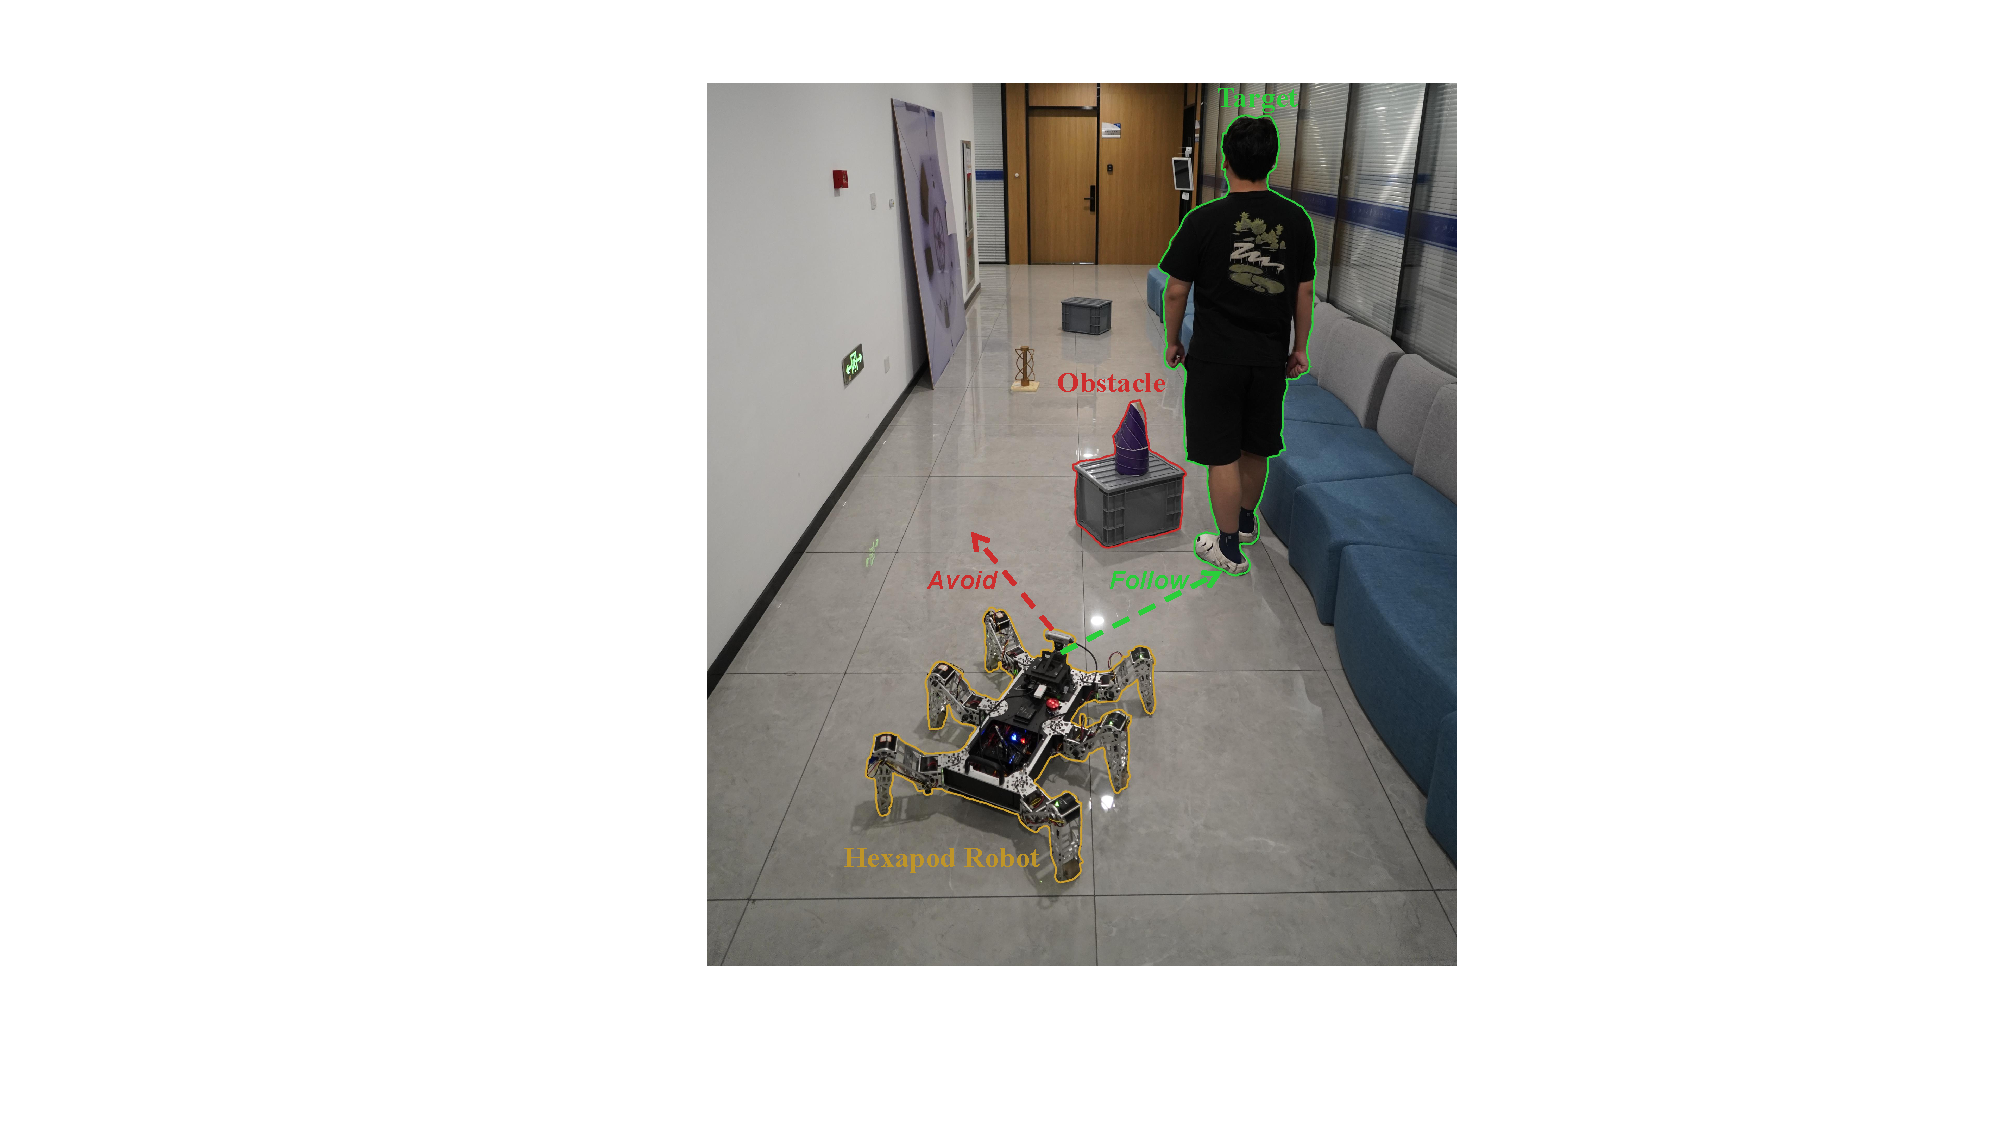
\includegraphics[width=.65\linewidth]{../完整TeX文件/figs/fig1_real_scene.pdf}%1
\or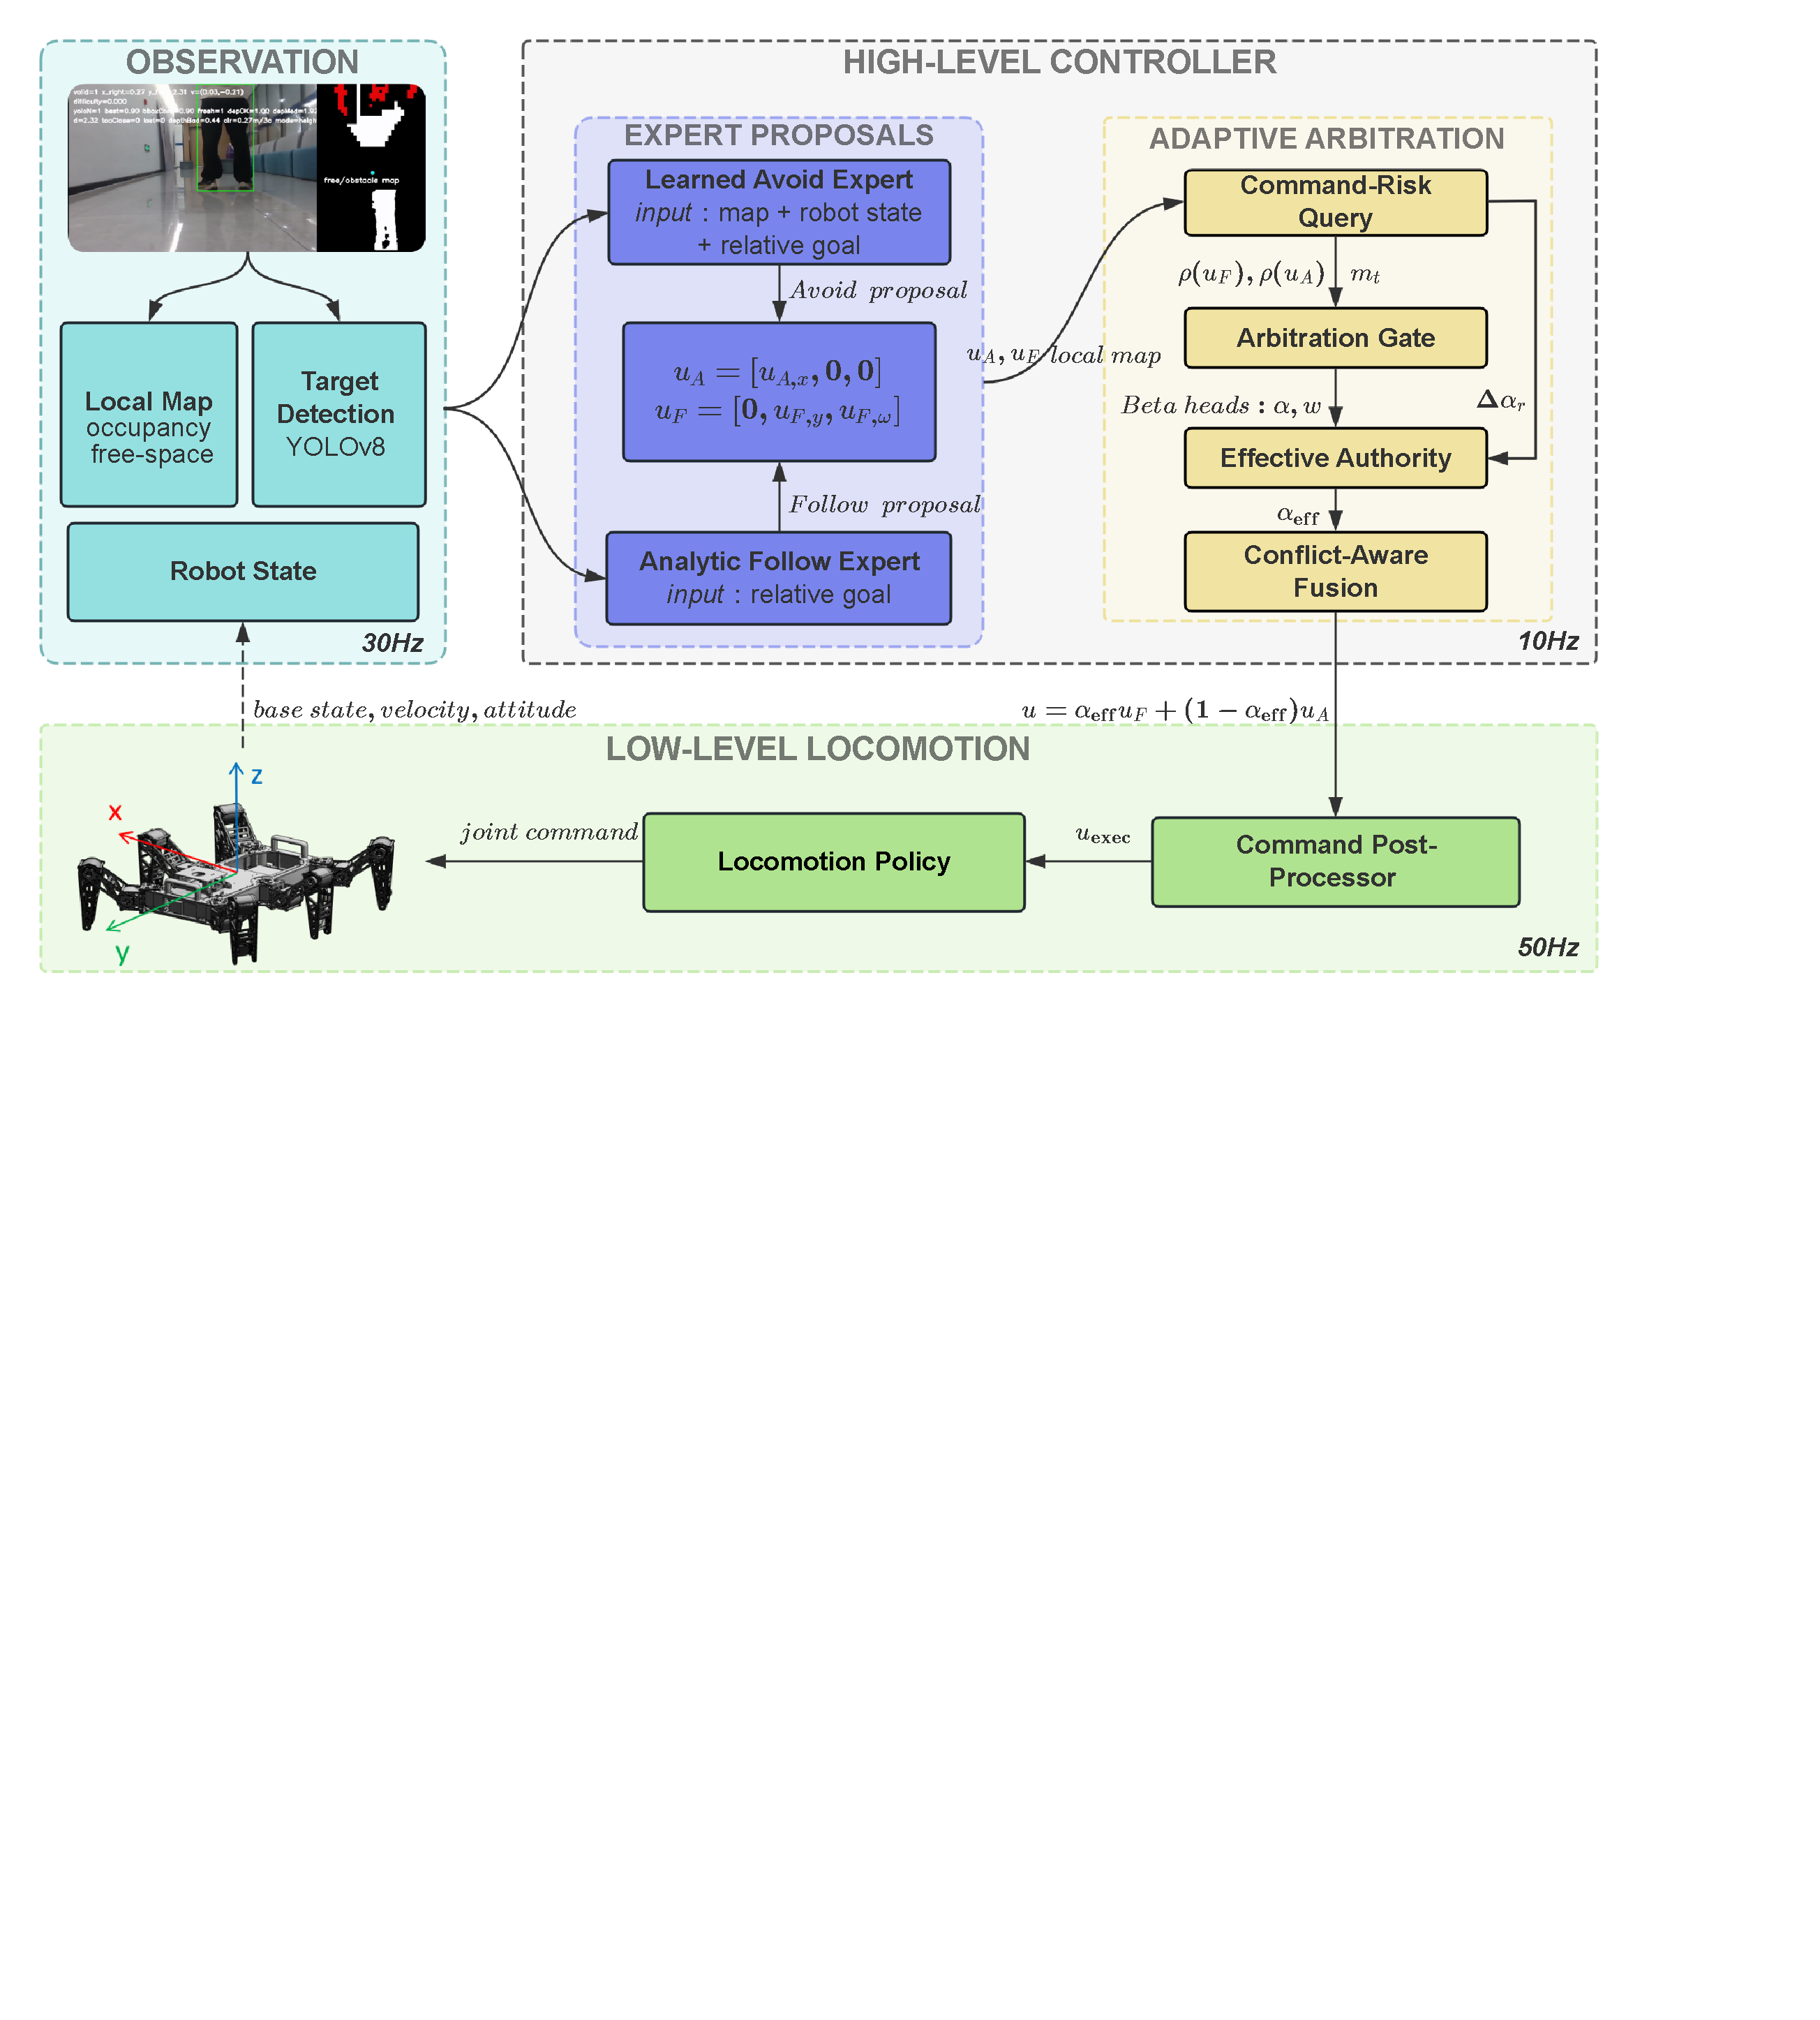
\includegraphics[trim=22.6bp 716.4bp 147.9bp 22.6bp,clip,width=.95\linewidth]{../完整TeX文件/figs/fig2_system.pdf}%2
\or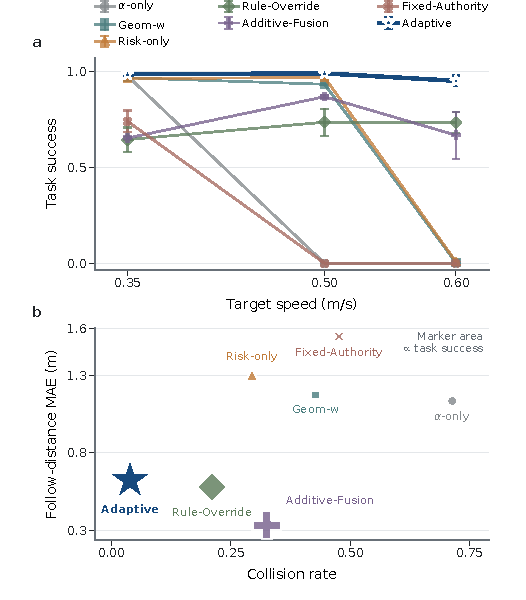
\includegraphics[width=.70\linewidth,trim=12bp 5bp 14bp 0bp,clip]{../完整TeX文件/figs/final_main_performance_nature.pdf}%3
\or\begin{minipage}[c]{.41\linewidth}\centering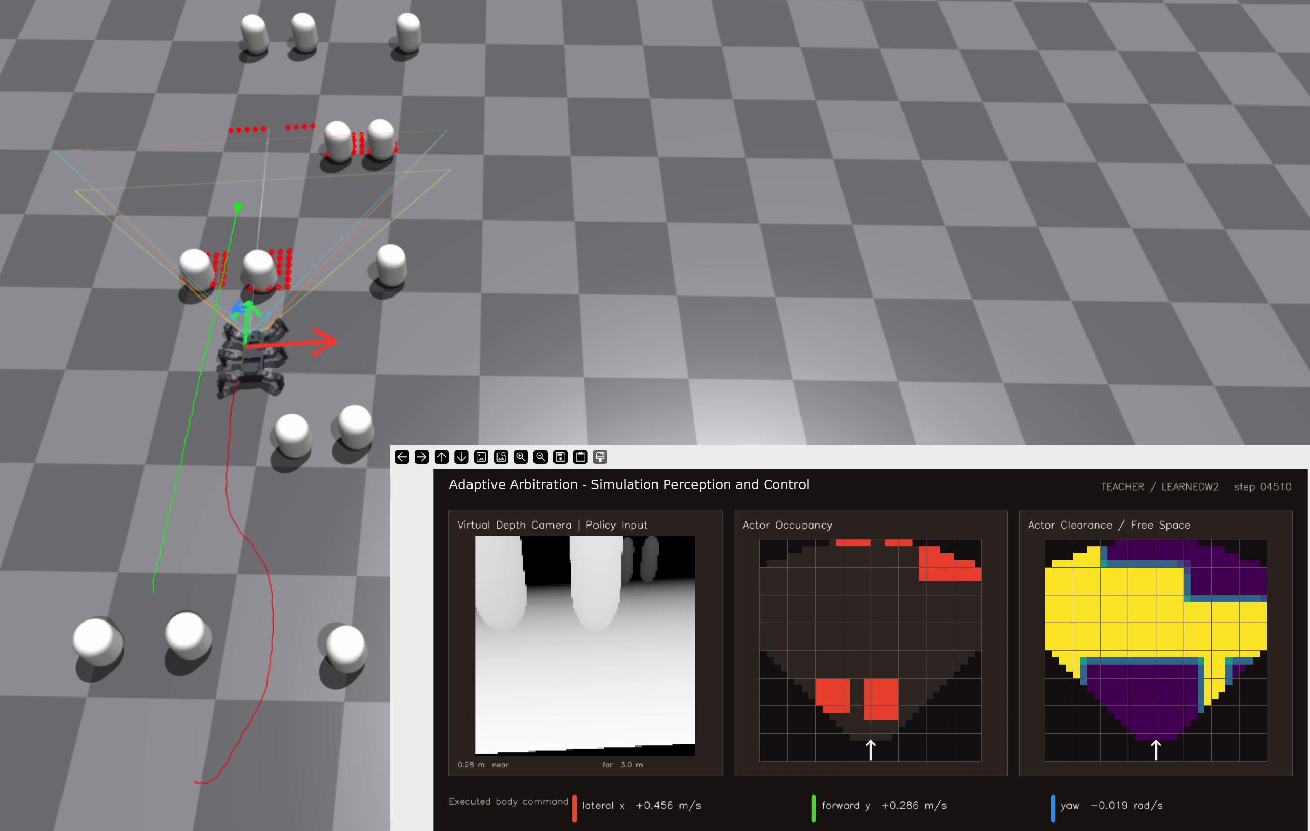
\includegraphics[width=\linewidth]{../完整TeX文件/figs/fig5_sim_overview_crop_adaptive.pdf}\par{\small(a)}\end{minipage}\hfill\begin{minipage}[c]{.55\linewidth}\centering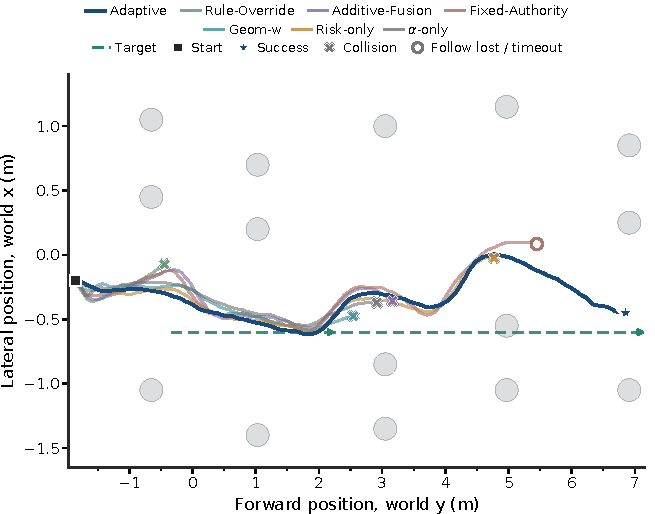
\includegraphics[width=\linewidth]{../完整TeX文件/figs/revision_heldout_mixed_v1_all_methods_trajectories_nature_refined.pdf}\par{\small(b)}\end{minipage}%4
\or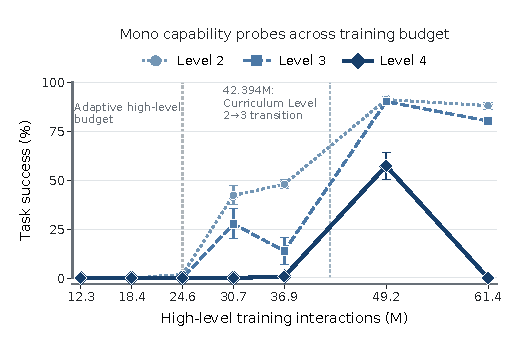
\includegraphics[width=.75\linewidth]{../完整TeX文件/figs/fig_mono_budget_capability_vertical.pdf}%5
\or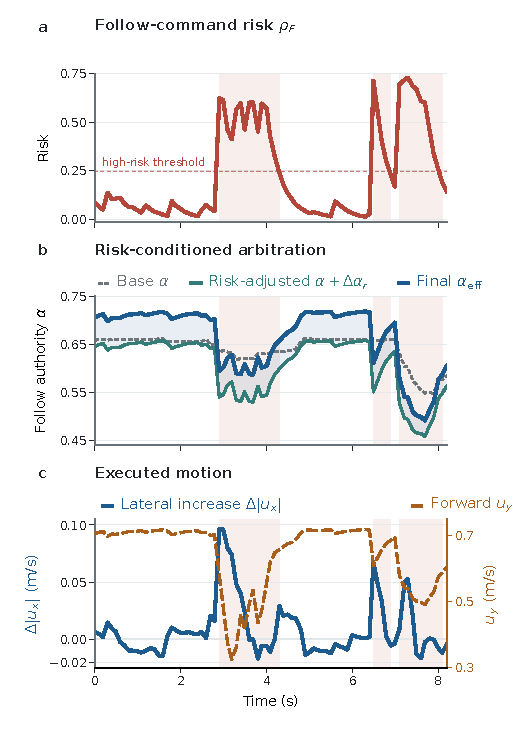
\includegraphics[width=.62\linewidth]{../完整TeX文件/figs/final_real_robot_arbitration_nature.pdf}%6
\or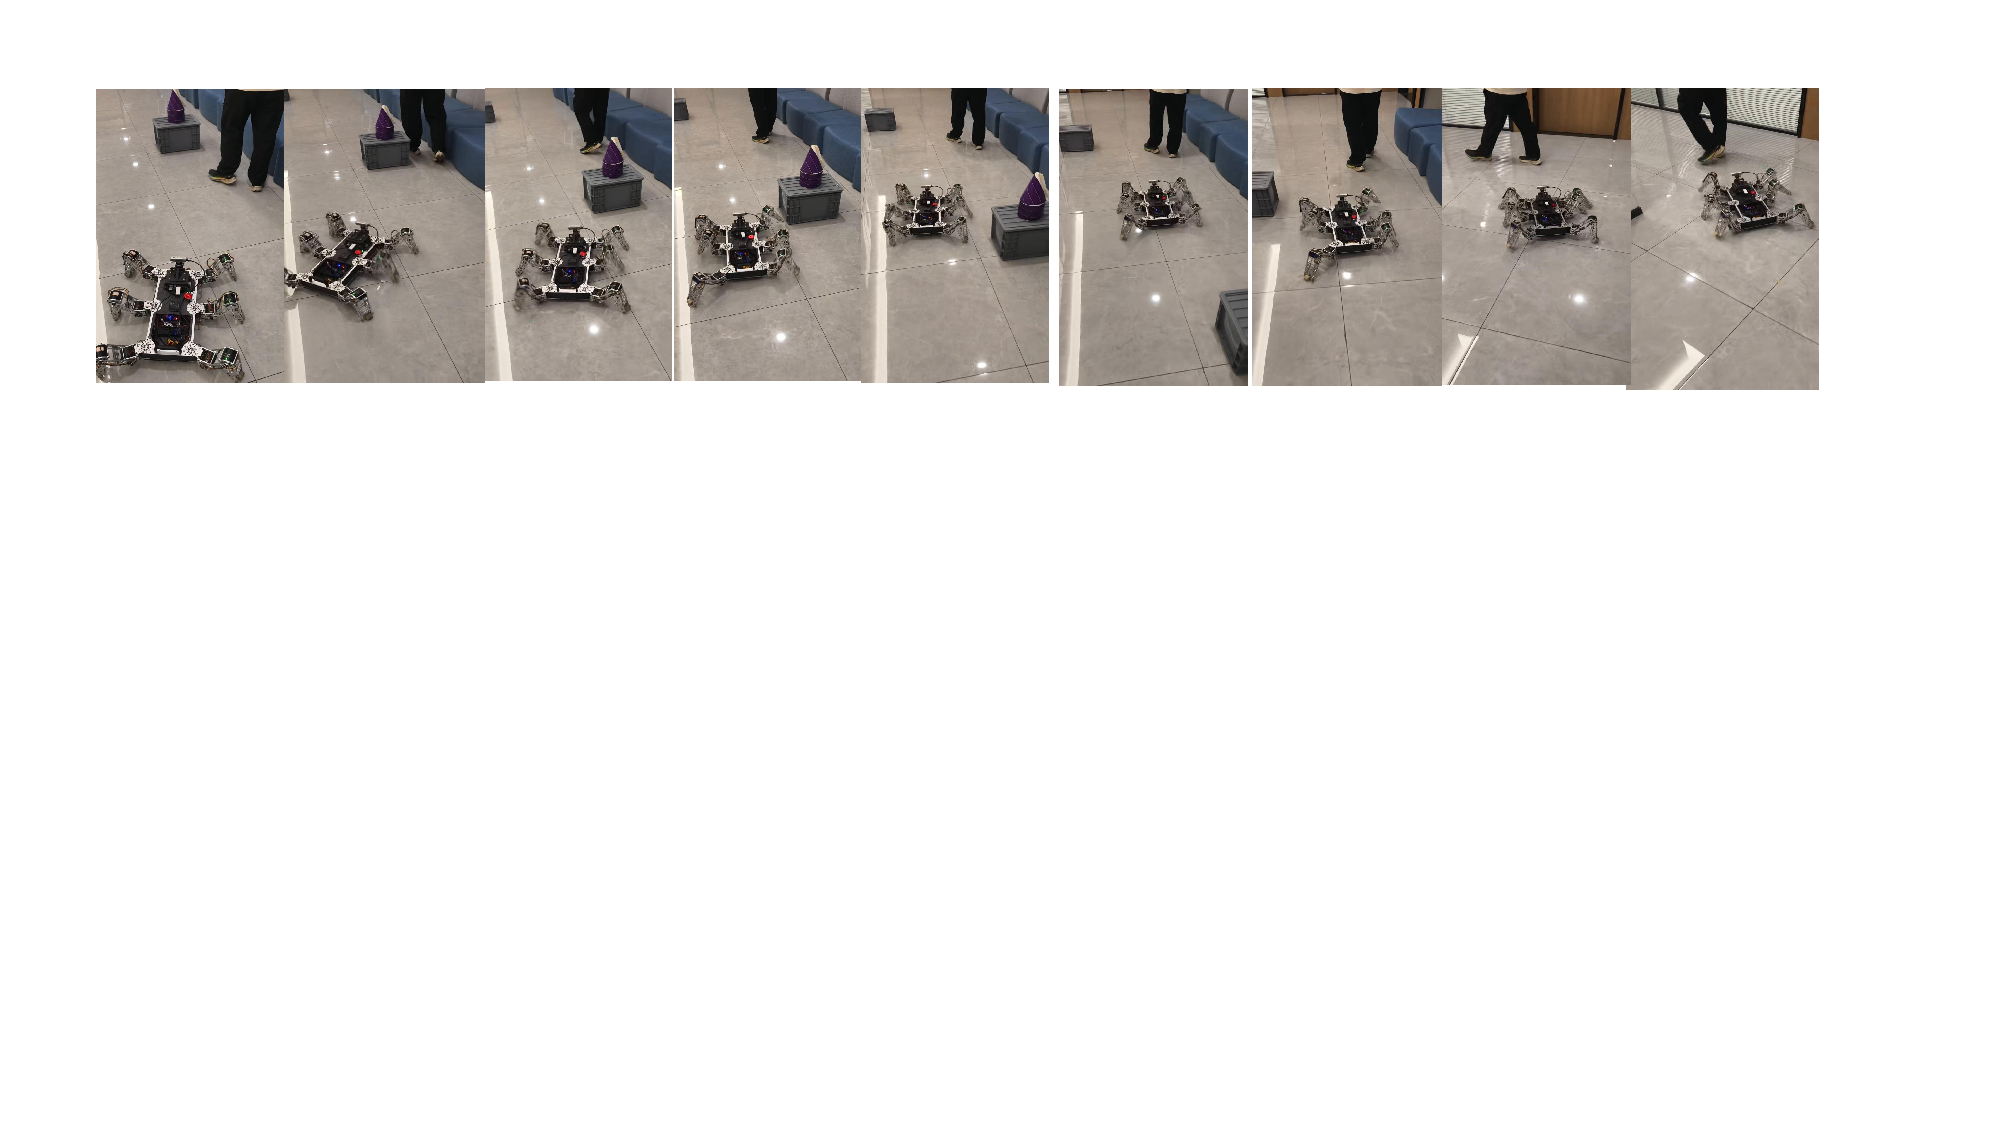
\includegraphics[width=.94\linewidth,height=.34\textheight,keepaspectratio]{../完整TeX文件/figs/fig4a_real_follow.pdf}\par{\small(a)}\smallskip
\includegraphics[width=.94\linewidth,height=.34\textheight,keepaspectratio]{../完整TeX文件/figs/revision_real_onboard.pdf}\par{\small(b)}%7
\fi
\caption{#2}\label{#3}\end{figure}}
\newcommand{\zhTable}[3]{%
\begin{table}[H]\centering\caption{#2}\label{#3}%
\begingroup\fontsize{9.5}{11}\selectfont\setlength{\tabcolsep}{2pt}\renewcommand{\arraystretch}{1.12}%
\csname zhTableFile#1\endcsname\endgroup\end{table}}
\expandafter\def\csname zhTableFile2\endcsname{\begin{tabular}{@{}llcccc@{}}
\toprule
速度 & 方法 & 成功率 [\%] $\uparrow$ & 障碍行进度 [\%] $\uparrow$ & 碰撞率 [\%] $\downarrow$ & 跟随距离 MAE [m] $\downarrow$ \\
\midrule
\multirow{7}{*}{\rotatebox{90}{$0.35$}} & $\alpha$-only & \ms{97.9}{0.5} & \ms{99.6}{0.1} & \ms{2.1}{0.5} & \ms{0.217}{0.001} \\
 & Geom-w & \ms{96.9}{1.4} & \ms{99.2}{0.6} & \ms{3.1}{1.4} & \ms{0.171}{0.001} \\
 & Risk-only & \ms{96.4}{1.2} & \ms{99.3}{0.2} & \ms{3.6}{1.2} & \ms{0.164}{0.001} \\
 & Rule-Override & \ms{64.6}{6.3} & \ms{82.1}{4.0} & \ms{34.6}{6.6} & \ms{0.164}{0.008} \\
 & Additive-Fusion & \ms{65.4}{1.2} & \ms{84.2}{1.0} & \ms{34.4}{1.4} & \ms{\mathbf{0.102}}{0.001} \\
 & \rev{Fixed-Authority} & \rev{\ms{74.2}{5.6}} & \rev{\ms{89.9}{3.0}} & \rev{\ms{24.5}{6.1}} & \rev{\ms{0.390}{0.009}} \\
 & \textbf{Adaptive} & \ms{\mathbf{98.7}}{0.9} & \ms{\mathbf{99.8}}{0.1} & \ms{\mathbf{1.3}}{0.9} & \ms{0.120}{0.000} \\
\midrule
\multirow{7}{*}{\rotatebox{90}{$0.50$}} & $\alpha$-only & \ms{0.0}{0.0} & \ms{93.0}{1.2} & \ms{30.7}{6.4} & \ms{0.969}{0.035} \\
 & Geom-w & \ms{93.5}{0.5} & \ms{97.2}{0.7} & \ms{6.5}{0.5} & \ms{0.430}{0.001} \\
 & Risk-only & \ms{97.1}{0.9} & \ms{99.0}{0.5} & \ms{2.9}{0.9} & \ms{0.405}{0.001} \\
 & Rule-Override & \ms{73.7}{7.1} & \ms{90.0}{2.8} & \ms{24.7}{7.3} & \ms{0.381}{0.013} \\
 & Additive-Fusion & \ms{87.0}{0.9} & \ms{94.6}{0.4} & \ms{12.5}{0.8} & \ms{\mathbf{0.177}}{0.002} \\
 & \rev{Fixed-Authority} & \rev{\ms{0.0}{0.0}} & \rev{\ms{43.6}{0.5}} & \rev{\ms{50.8}{4.1}} & \rev{\ms{1.220}{0.020}} \\
 & \textbf{Adaptive} & \ms{\mathbf{99.2}}{0.8} & \ms{\mathbf{99.9}}{0.2} & \ms{\mathbf{0.8}}{0.8} & \ms{0.355}{0.003} \\
\midrule
\multirow{7}{*}{\rotatebox{90}{$0.60$}} & $\alpha$-only & \ms{0.0}{0.0} & \ms{79.4}{0.9} & \ms{71.4}{3.6} & \ms{1.133}{0.012} \\
 & Geom-w & \ms{0.3}{0.5} & \ms{74.6}{1.8} & \ms{42.7}{8.4} & \ms{1.172}{0.015} \\
 & Risk-only & \ms{0.8}{0.8} & \ms{71.5}{0.2} & \ms{29.4}{7.1} & \ms{1.305}{0.031} \\
 & Rule-Override & \ms{73.4}{5.5} & \ms{86.1}{2.7} & \ms{21.1}{4.8} & \ms{0.582}{0.019} \\
 & Additive-Fusion & \ms{66.9}{12.3} & \ms{87.4}{5.0} & \ms{32.6}{12.6} & \ms{\mathbf{0.334}}{0.040} \\
 & \rev{Fixed-Authority} & \rev{\ms{0.0}{0.0}} & \rev{\ms{39.9}{0.1}} & \rev{\ms{47.7}{2.8}} & \rev{\ms{1.549}{0.004}} \\
 & \textbf{Adaptive} & \ms{\mathbf{95.3}}{2.8} & \ms{\mathbf{98.5}}{0.8} & \ms{\mathbf{3.9}}{2.7} & \ms{0.623}{0.004} \\
\bottomrule
\end{tabular}
}
\expandafter\def\csname zhTableFile3\endcsname{\begin{tabular}{lccccc}
\toprule
速度 & 成功率 $\uparrow$ & 障碍行进度 $\uparrow$ & 碰撞率 $\downarrow$ & 跟随距离 MAE [m] $\downarrow$ &
$\Delta\alpha_w$ （预测） \\
\midrule
$0.35$ & $0.974$ & $0.993$ & $0.023$ & $0.176$ & $0.066$ \\
$0.50$ & $0.982$ & $0.992$ & $0.016$ & $0.438$ & $0.067$ \\
$0.60$ & $0.000$ & $0.739$ & $0.133$ & $1.463$ & $0.066$ \\
\bottomrule
\end{tabular}
}
\expandafter\def\csname zhTableFile4\endcsname{\begin{tabular}{lcccc}
\toprule
策略 & 预算（M） & 0.35 & 0.50 & 0.60 \\
\midrule
Adaptive & 24.576 & \ms{98.7}{0.9} & \ms{99.2}{0.8} & \ms{95.3}{2.8} \\
Mono 2000 & 24.576 & \ms{0.0}{0.0} & \ms{0.0}{0.0} & \ms{0.0}{0.0} \\
Mono 4000 & 49.152 & \ms{57.3}{6.7} & \ms{94.5}{0.0} & \ms{0.0}{0.0} \\
Mono 5000 & 61.440 & \ms{0.0}{0.0} & \ms{93.0}{2.7} & \ms{1.3}{0.9} \\
\bottomrule
\end{tabular}
\par\smallskip{\footnotesize Adaptive：12.288M 次 Avoid 交互＋12.288M 次门控交互（不计共用底层训练）；Mono 使用一个训练种子。数值为三个评测种子上的均值 $\pm$ 样本标准差；每一行 Mono 在各速度下使用同一检查点。}\par
}
\expandafter\def\csname zhTableFile5\endcsname{\begin{tabular}{llcccc}
\toprule
搜索偏好 & 速度 & 成功率 $\uparrow$ & 碰撞率 $\downarrow$ &
障碍行进度 $\uparrow$ & 跟随距离 MAE [m] $\downarrow$ \\
\midrule
\multirow{2}{*}{偏重安全}
 & $0.35$ & $0.053$ & $0.612$ & $0.138$ & $0.678$ \\
 & $0.60$ & $0.000$ & $0.838$ & $0.000$ & $1.028$ \\
\multirow{2}{*}{均衡}
 & $0.35$ & $0.026$ & $0.938$ & $0.188$ & $0.375$ \\
 & $0.60$ & $0.000$ & $0.969$ & $0.375$ & $0.592$ \\
\multirow{2}{*}{偏重跟踪}
 & $0.35$ & $0.082$ & $0.744$ & $0.344$ & $0.528$ \\
 & $0.60$ & $0.000$ & $0.881$ & $0.500$ & $0.690$ \\
\bottomrule
\end{tabular}
}
\expandafter\def\csname zhTableFile6\endcsname{\begin{tabular*}{\columnwidth}{@{\extracolsep{\fill}}llccccc@{}}
\toprule
方法 & 场景 & 试验次数 & 成功次数 & 碰撞 & 目标丢失 & 成功率 \\
\midrule
Adaptive & 交错障碍行 & $20$ & $19$ & $1$ & $0$ & $95\%$ \\
Rule-Override & 交错障碍行 & $20$ & $12$ & $6$ & $2$ & $60\%$ \\
Adaptive & 目标急转弯 & $20$ & $18$ & $1$ & $1$ & $90\%$ \\
Adaptive & 总体 & $40$ & $37$ & $2$ & $1$ & $92.5\%$ \\
\bottomrule
\end{tabular*}
}
\renewenvironment{quote}{\list{}{\rightmargin=2em\leftmargin=2em}\item\relax\color{reviewgray}\normalfont}{\endlist}
\newcommand{\reviewcomment}[2]{\par\Needspace{4\baselineskip}\noindent\textbf{意见 #1：#2}\par\smallskip}
\newcommand{\response}{\par\noindent\textbf{回复。}\quad}
\newcommand{\location}[1]{\par\smallskip\noindent{\small\itshape 修改位置：#1}\par\medskip}
\newcounter{zhbookmark}
\makeatletter
\let\zh@oldsection\section
\renewcommand{\section}{\@ifstar{\zh@starsection}{\zh@numberedsection}}
\newcommand{\zh@starsection}[1]{\stepcounter{zhbookmark}\pdfbookmark[1]{#1}{zhsec\arabic{zhbookmark}}\zh@oldsection*{#1}}
\newcommand{\zh@numberedsection}[1]{\zh@oldsection{#1}}
\let\zh@oldsubsection\subsection
\renewcommand{\subsection}{\@ifstar{\zh@starsubsection}{\zh@numberedsubsection}}
\newcommand{\zh@starsubsection}[1]{\stepcounter{zhbookmark}\pdfbookmark[2]{#1}{zhsub\arabic{zhbookmark}}\zh@oldsubsection*{#1}}
\newcommand{\zh@numberedsubsection}[1]{\zh@oldsubsection{#1}}
\makeatother
\begin{document}
\pdfbookmark[0]{中文论文}{zh-main}
\begin{center}\small 中文阅读版；依据 2026-10-01 英文修订稿及回复信翻译。公式、数据和文献条目保留原文；图内英文附中文对照；回复中修改位置指向英文修订稿。\end{center}
\begin{center}
{\LARGE\bfseries 通行性不匹配条件下目标跟随的指令空间自适应仲裁}\par
\end{center}
\begin{abstract}
足式机器人在杂乱环境中跟随行人时，可能遇到行人能够通过、机器人却无法安全通过的通道。这种通行性不匹配使目标恢复与障碍间隙之间产生冲突。我们提出一种指令空间自适应仲裁框架，协调解析生成的前向—偏航跟随提议与预训练的横向避障提议。学习仲裁门控根据风险调整两者的相对控制权，同时固定两个专家和运动策略，使学习集中于行为协调。在留出评测中，该方法在 $0.60\,\mathrm{m/s}$ 下实现了 $95.3\%$ 的任务成功率，该速度比训练最高速度高 $20\%$。结合机载目标检测和双目深度，该方法在交错行走廊和急转弯走廊的 40 次实机试验中成功 37 次。与加性融合、固定控制权和单体 PPO 的比较支持了情境相关控制权分配在所测条件下的价值。
\end{abstract}

\section{引言}
运动中的行人可以穿过某些间隙，而足式机器人的步态包络无法安全通过这些间隙（图~\ref{fig:teaser}）。这种\emph{通行性不匹配}使避碰与目标保持相互耦合：跟踪行人可能减小障碍间隙，而避障可能导致目标丢失。我们研究如何随着这一冲突的变化，在 Follow（跟随）和 Avoid（避障）提议之间分配控制权。

所提出的仲裁框架在正交指令子空间中组合解析 Follow 提议与学习得到的 Avoid 提议（图~\ref{fig:system}）。门控利用沿各提议方向的障碍风险分配两者的控制权。专家和预训练运动策略保持固定，使学习集中于它们之间的协调。

\zhfigure{1}{杂乱环境中六足机器人目标跟随的真实走廊场景。目标能够通过的间隙可能不足以容纳机器人包含腿部的包络，从而在目标恢复与碰撞规避之间产生冲突。}{fig:teaser}

六足机器人能够完成该分解所需的横向运动，其固定的 18 关节运动策略负责实现指令。仲裁使用高层速度，而不使用六足机器人特有的关节观测。交错障碍行构成一种受控压力测试：目标持续前进时，机器人需要侧移通过连续障碍行。

\noindent\textbf{贡献。}
\begin{itemize}
\item \textbf{通行性不匹配的指令空间表述。}我们将运动目标保持与局部碰撞规避之间的冲突，表述为指令空间中的连续控制权分配问题。
\item \textbf{风险条件化自适应仲裁。}风险条件化门控融合正交指令子空间中固定的 Follow 和 Avoid 提议。有界的原始凸组合经过各方法共用的后处理，再由固定运动策略执行。
\item \textbf{仲裁的受控验证。}仲裁变体之间的比较复用相同专家，推理消融复用同一检查点，从而保持专家能力和运动能力不变。留出仿真评测和实机试验量化了安全与跟随之间的权衡。
\end{itemize}

\section{相关工作}
\emph{跟随、避障与敏捷运动。}行人跟随通常被表述为移动机器人跟踪与局部导航问题~\cite{ref:personfollowing}，而人机交互（HRI）研究还考虑可见性、人际距离及社会可接受的运动~\cite{ref:socialfollow}。He 等人~\cite{ref:abs}采用到达—避障表述，协调敏捷行为与恢复行为，实现朝向静态目标的无碰撞运动；Miki 等人~\cite{ref:miki}利用外感知和本体感知输入学习感知驱动的运动。我们的重点是在局部避障过程中持续跟踪运动目标。

\emph{规划、安全与专家仲裁。}动态窗口方法对短时域内的间隙和推进进行评分~\cite{ref:dwa}；我们在第~VI-D 节纳入一种采用相同指令接口的 DWA 类替代方法。控制屏障函数将约束编码到在线二次规划中~\cite{ref:cbf}。约束策略优化在显式代价约束下最大化回报~\cite{ref:cpo}；我们的训练通过奖励塑形表达跟随与障碍间隙之间的权衡。在行为组合方面，经典混合专家方法学习门控函数~\cite{ref:moe}，而 MELA 组合专家网络参数~\cite{ref:mela}。Scheidemann 等人~\cite{ref:leaderfollow}通过 RMP 加速度与度量组合领航者跟随和避障。共享控制方法依据情境融合策略~\cite{ref:policyblend}，残差强化学习则学习加性动作修正~\cite{ref:residualrl}。相比之下，我们的门控学习固定 Follow 和 Avoid 速度提议之间的标量控制权。固定两个专家，使门控训练集中于何时以及在多大程度上偏向各行为。

\section{问题表述}
\textbf{A. 场景设定。}受控压力测试采用具有侧向通道的障碍行（图~\ref{fig:teaser}）。高层控制器以 $10\,\mathrm{Hz}$ 输出速度指令 $u=[u_x,u_y,u_\omega]^\top$（横向、前向、偏航），由固定的底层运动策略以 $50\,\mathrm{Hz}$ 实现。机器人感知局部占据—自由空间地图及目标相对状态；不使用全局地图。

\textbf{B. 正交指令分解。}我们将跟随与避障分配到正交指令子空间。Follow 专家作用于前向—偏航子空间，Avoid 专家作用于横向子空间，
\begin{equation}
\mathcal{U}_F=\{[0,u_y,u_\omega]^\top\},\quad
\mathcal{U}_A=\{[u_x,0,0]^\top\},
\end{equation}
因此 $\mathbb{R}^3=\mathcal{U}_F\oplus\mathcal{U}_A$，且 $\mathcal{U}_F\perp\mathcal{U}_A$。Follow 指令 $\uF=[0,u_{F,y},u_{F,\omega}]\in\mathcal{U}_F$ 通过解析方式计算；学习得到的 Avoid 专家生成原始指令，再投影到横向子空间，得到 $\uA=[u_{A,x},0,0]\in\mathcal{U}_A$。由于偏航位于 Follow 子空间，非零的 Follow 控制权会在横向避障时保留部分朝向目标的偏航，使机器人在侧移过程中更容易持续面向目标。

\textbf{C. 冲突。}这些提议可以在代数上相加，但它们的执行效果受机器人足迹、障碍几何、运动动力学、指令限制和目标可见性共同耦合。因此，跟踪可能减小间隙，而避障可能增大目标误差。仲裁随着这一冲突的变化调节提议的相对控制权。

\textbf{D. 任务成功与诊断量。}我们将事件层面的成功与轨迹诊断量区分开。只有当任务完成时机器人已通过最后一行障碍、处于 $[1.0,2.2]\,\mathrm{m}$ 的跟随距离区间内，且在整个回合中均未发生碰撞，该次试验才成功。我们还报告轨迹诊断量：跟随距离 MAE（在各高层时间步上计算 $|\mathrm{dist}(\text{target},\text{robot})-d_{\mathrm{des}}|$ 的均值，其中 $d_{\mathrm{des}}=1.5\,\mathrm{m}$）、L1（无碰撞）、L2（保持目标：跟随距离 MAE $\le0.5\,\mathrm{m}$ 且目标处于视野内的比例 $\ge0.90$），以及 L3（通过最后一行障碍）。距离条件在任务完成时检查；跟随距离 MAE 与 L2 概括整条轨迹上的跟踪表现，L2 不是额外的成功条件。

\zhfigure{2}{指令空间中的自适应仲裁。机载感知提供局部占据—自由空间地图与目标相对状态（YOLOv8）。解析 Follow 专家提出前向—偏航运动，学习得到的 Avoid 专家提出横向运动，方向风险及其标量记忆作为仲裁门控的输入。门控计算 $\alphaeff$ 以融合指令，随后经过共用的指令后处理和固定运动策略。图中频率为部署频率：感知 30 Hz、仲裁 10 Hz、运动控制 50 Hz。}{fig:system}
\figtranslation{图中文字对照：Observation：观测；High-level controller：高层控制器；Local Map：局部地图；occupancy/free-space：占据／自由空间；Target Detection：目标检测；Robot State：机器人状态；Expert Proposals：专家提议；Learned Avoid Expert：学习避障专家；Analytic Follow Expert：解析跟随专家；input：输入；map + robot state + relative goal：地图＋机器人状态＋相对目标；Avoid/Follow proposal：避障／跟随提议；Adaptive Arbitration：自适应仲裁；Command-Risk Query：指令风险查询；Arbitration Gate：仲裁门控；Beta heads：Beta 输出头；Effective Authority：有效控制权；Conflict-Aware Fusion：冲突感知融合；Low-level Locomotion：底层运动控制；Command Post-Processor：指令后处理器；Locomotion Policy：运动策略；joint command：关节指令；base state, velocity, attitude：机体状态、速度与姿态。}

\section{方法}
\label{sec:method}
控制器由固定运动策略、正交专家提议和学习仲裁门控组成（图~\ref{fig:system}）。

\textbf{A. Follow 专家（解析式）。}Follow 专家根据表示目标相对于机器人位置的二维相对目标，解析计算 $\uF=[0,u_{F,y},u_{F,\omega}]$，并采用带迟滞的先转向后前进规则：当方位角的绝对值超过 $0.35\,\mathrm{rad}$ 时，抑制前向项，机器人原地转向；当方位角的绝对值降至 $0.18\,\mathrm{rad}$ 以下时，恢复前进。

\textbf{B. Avoid 专家（学习式）。}Avoid 在随机化障碍布局中独立预训练。通道难度随阶段变化，环境提供前向运动，Follow 不参与。预训练的演员网络保留三个指令输出，而仲裁仅使用其横向均值作为冻结的 Avoid 提议 $\uA$（观测与网络结构见第~IV-F 节及表~\ref{tab:architecture}）。

奖励鼓励前向推进和方向间隙改善，惩罚横向指令的幅值与变化，并在两个横向备选方向均足够通畅时提供微弱的方向偏好。在 $\Delta t=0.1\,\mathrm{s}$ 时，稠密奖励为
\begin{equation}
\begin{aligned}
r_t^A={}&\Delta y+0.03q_0(q_0-q_u)-0.005|u_x^{\mathrm{raw}}|\\
&-0.01|u_{x,t}^{\mathrm{exec}}-u_{x,t-1}^{\mathrm{exec}}|
+0.0005Gp\tfrac{u_x^{\mathrm{exec}}}{u_{x,\max}},
\end{aligned}
\label{eq:avoid_reward}
\end{equation}
其中，$\Delta y$ 是前向位移，$q_j=\mathrm{clip}((0.57-d_j)/0.57,0,1)$，$j=0,u$。距离 $d_0,d_u$ 在动作执行前的同一地图上，分别沿正前方方向与原始指令方向，使用半角为 $25^\circ$ 的锥形区域查询。上标 raw/exec 分别表示处理前／后的指令；$u_{x,\max}$ 为横向限值。偏好 $p$ 是有效前向目标方向的归一化横向分量。只有在 Avoid 阶段 1 之后，且偏好有效、$\Delta y>0$、$d_0<0.57$、$d_L,d_R\ge0.57$、$|d_L-d_R|\le0.10$ 时，指示量 $G=1$（距离单位为米）；否则 $G=0$。这里，$d_L,d_R$ 分别查询横向指令 $\pm u_{x,\max}$ 与所提供前向指令组合后的方向。奖励不使用行索引、间隙中心或通道模板。

终止奖励替代 $r_t^A$：机器人中心在未发生失败的情况下越过布局出口线时奖励为 $+2$；发生碰撞、包络侵入、跌倒或倾角／高度违规时奖励为 $-20$，且失败判定优先。超时结束回合，但不施加失败惩罚。横向避障假设前方可以观测到可行的绕行通道。

\textbf{C. 方向指令风险。}门控接收机器人固定坐标系中的双通道局部占据—自由空间地图。该地图表示为 $32\times32$ 栅格，覆盖前方 $3\,\mathrm{m}\times3\,\mathrm{m}$ 区域，原点位于相机安装位置。占据通道标记被占据的单元。自由空间通道是一个无量纲分数：对占据区域进行膨胀，生成自由空间掩膜，将其与 $3\times3$ 局部平均值逐单元取最大值，再屏蔽被占据及未观测单元；它不是以实际距离为单位的距离场。仿真中，占据区域膨胀采用 $7\times7$ 方形核。膨胀半径依据六足机器人的实体测量选取，以考虑机身尺寸以及行走过程中腿部运动带来的额外横向范围。对于每个具有非零平移的提议，在以 $\mathrm{atan2}(u_x,u_y)$ 为中心、半角为 $25^\circ$ 的锥形区域中，查询地图原点到占据通道中最近占据单元的距离 $d$（若锥形区域内未观测到占据单元，则 $d=3.0\,\mathrm{m}$）。平移接近零时，仿真中的查询回退为局部地图内占据单元的最小距离。两种查询均不评估偏航运动的扫掠范围。侧移可利用前方已观测到的绕行空间提前开始，但查询锥内未观测到障碍，并不表示整条侧向路径都已确认畅通。风险为
\begin{equation}
\rho(u)=1-\mathrm{clip}\!\left(\tfrac{d-d_{\mathrm{safe}}}{d_{\mathrm{free}}-d_{\mathrm{safe}}},0,1\right),
\end{equation}
其中 $d_{\mathrm{safe}}=0.27\,\mathrm{m}$，$d_{\mathrm{free}}=0.57\,\mathrm{m}$。这些固定阈值定义的是方向接近程度分数，而不是机器人扫掠体的间隙。$25^\circ$ 半角是定义方向查询邻域的固定启发式参数；不使用速度缩放或制动距离模型。

对于各提议，$\rho_F=\rho(\uF)$，$\rho_A=\rho(\uA)$。\emph{按距离衰减的风险记忆。}为保留近期危险信息，标量风险记忆随机体前向位移衰减，在纯横向运动或停止时不衰减：
\begin{equation}
\begin{aligned}
m_t &= \max\!\big(\rho_{F,t},m_{t-1}e^{-\Delta s/L_{\mathrm{clear}}}\big),\\
\Delta s &= \max(v_{y,t}^{\mathrm{body}},0)\,\Delta t,
\end{aligned}
\end{equation}
其中 $L_{\mathrm{clear}}=0.40\,\mathrm{m}$。该标量作为派生冲突特征输入门控。瞬时风险反映当前地图观测；$m_t$ 保留的是标量危险信号，而不是障碍地图。

\textbf{D. 门控与冲突感知融合。}单一仲裁门控通过 Beta 输出头生成基础 Follow 控制权 $\alpha\in(0,1)$ 和学习冲突变量 $w\in(0,1)$。门控结合局部几何、机器人与目标状态，以及依赖于提议的冲突特征；具体观测在第~IV-F 节列出。学习得到的有符号调制项与解析风险修正项为
\begin{align}
\Delta\alpha_w &= \lambda\,\mathrm{deadband}(2w-1),\quad
\Delta\alpha_r = \gamma(\rAdir-\rFdir), \\
\alphaeff &= \mathrm{clip}\!\left(\alpha+\Delta\alpha_w+\Delta\alpha_r,0,1\right),
\end{align}
其中 $\lambda=0.30$、$\gamma=0.15$；当 $|z|>0.05$ 时，$\mathrm{deadband}(z)=z$，否则为 $0$。融合指令为
\begin{equation}
u = \alphaeff\,\uF + (1-\alphaeff)\,\uA.
\label{eq:fusion}
\end{equation}
在死区之外，$w>0.5$ 通过 $\Delta\alpha_w$ 增强跟随，$w<0.5$ 则抑制跟随。在调制生效且未饱和的区域，$\partial\alphaeff/\partial w=2\lambda=0.60$；在死区内或限幅后，该导数为零。这些增益将限幅前学习修正项和解析修正项的幅度分别限制在 $0.30$ 和 $0.15$ 内。

\textbf{E. 底层运动接口。}固定运动策略以 $50\,\mathrm{Hz}$ 跟踪高层指令，各方法共用这一策略。执行前，所有方法均采用相同的幅值限幅、用于约束指令变化的变化率限制，以及基于间隙的缩放，以在接近障碍时减弱平移。

\textbf{F. 训练过程。}首先使用 RSL-RL~\cite{ref:rudin} 预训练并冻结以速度指令为条件的六足运动策略，奖励项包括相机稳定性和平滑冲击。Avoid 也保持冻结（第~IV-B 节），此后仅训练仲裁门控。权重为 $0.05$ 的辅助二元交叉熵损失，在明显应偏向避障的状态下鼓励 $w=0$：一类是障碍行尚未释放，且满足 $\rFdir>0.25$、$\rFdir-\rAdir>0.05$、指令余弦值 $<0.5$ 的情形；另一类是不受行释放条件限制、满足 $\rFdir>0.45$、$\rFdir-\rAdir>0.15$、指令余弦值 $<0.3$ 的全局情形。

Avoid 专家、运动策略和门控均使用 Isaac Gym~\cite{ref:isaac} 中相同的六足机器人模型；运动策略使用 RSL-RL，两个学习型高层策略使用 PPO~\cite{ref:ppo}。课程包含四个等级，同时将障碍行数从两行变到五行、将目标速度从 $0.25$ 变到 $0.50\msec$；每个回合内速度固定。在 $120{,}000$ 个回合中，采样逐步偏向更困难的等级，同时保留较简单回合。五行训练布局使用两个镜像模板，左右通道交替，障碍位置施加最大 $\pm0.06\,\mathrm{m}$ 的独立扰动；第~V-A 节介绍留出评测。训练障碍为静态，半径为 $0.15\,\mathrm{m}$、高度为 $0.50\,\mathrm{m}$；接触摩擦系数在 $[0.4,0.8]$ 内随机化。训练时，策略接收由仿真障碍几何栅格化得到、并限制在 D435i 双目视野内的局部占据—自由空间地图，而不是渲染深度。

\begin{table}[htbp]
\centering\small
\caption{Avoid 专家与仲裁门控的网络结构。两者的地图编码器结构相同、权重独立；参数量包含训练时使用的评论家网络}
\label{tab:architecture}
\renewcommand{\arraystretch}{1.25}\setlength{\tabcolsep}{4pt}
\begin{tabular}{@{}p{0.13\linewidth}p{0.405\linewidth}p{0.405\linewidth}@{}}
\toprule
模块 & Avoid 专家 & 仲裁门控\\\midrule
地图编码器 & \multicolumn{2}{p{0.83\linewidth}@{}}{双通道局部占据／自由空间地图＋两个归一化坐标通道；卷积 $4\to32\to64\to128$（$3\times3$，步长 $2/2/1$，填充 1，ELU）；自适应 $4\times4$ 平均池化；全连接层 $2048\to128$。}\\
标量编码器 & 状态 MLP $14\to64\to64\to64$；目标 MLP $2\to32\to32$（ELU）。 & 状态 MLP $13\to64\to64\to64$；目标／冲突 MLP $18\to32\to32$（ELU；总计 31 个标量输入）。\\
融合 & \multicolumn{2}{p{0.83\linewidth}@{}}{拼接 $128+64+32+1=225$；MLP $225\to256\to256$（ELU）。评测门控的一维难度输入固定为零。}\\
演员输出头 & 均值 $256\to64\to3$；标准差 $256\to64\to3$（Softplus）；执行横向均值。 & 四个 $256\to64\to1$ 的 Softplus 浓度参数输出头；构成 $\alpha,w$ 的两个 Beta 分布；评测时使用 Beta 分布均值。\\
评论家／参数量 & 价值 $256\to64\to1$；1,029,575 个参数。 & 价值 $256\to64\to1$；1,063,237 个参数。\\
\bottomrule\end{tabular}
\end{table}

表~\ref{tab:architecture} 汇总了网络结构；评论家使用独立的编码器和主干网络。门控的 13 维机器人状态包括世界坐标系平面位置、偏航角、机体系平面速度、偏航角速度、高度、横滚／俯仰角、上一时刻的基础控制权 $\alpha$，以及上一条指令。Avoid 将控制权槽位固定为零，并追加强制前向速度（构成 14 维状态）；其地图和二维相对目标为独立输入。门控的 18 维目标／冲突向量包括相对目标、Follow／Avoid 提议及其差值（9）、风险 $\rho_F,\rho_A$、风险记忆 $m_t$、平移指令余弦 $c$、冲突分数 $\max(\rho_F-\rho_A,0)(1-c)/2$，以及两个归一化间隙 $\mathrm{clip}(d/(3\,\mathrm{m}),0,1)$。当任一平移提议的范数不超过 $10^{-6}$ 时，令 $c=1$。

两个高层阶段各使用 1,000 次迭代（12.288M 次交互），共计 24.576M 次；不计入共用且冻结的底层运动策略训练。门控 PPO 使用 256 个环境，每次迭代 48 步；Avoid 使用 512 个环境，每次迭代 24 步。门控每次迭代优化五个 epoch，小批量大小为 12,288，学习率为 $6\times10^{-5}$，熵系数为 0.04，截断比率为 0.05。门控训练将障碍行进度、跟随距离、成功以及碰撞／失败／时间奖励，与 $w$ 辅助损失相结合。行释放信息仅提供辅助训练标签；演员网络接收的则是标量风险记忆。

\textbf{G. 结构性质与适用范围。}原始融合指令位于提议的凸包内。令 $u_{\mathrm{nom}}=\alpha\uF+(1-\alpha)\uA$，$\delta u=u-u_{\mathrm{nom}}$，则
\begin{equation}
\begin{aligned}
\delta u &= (\alphaeff-\alpha)(\uF-\uA),\\
\|\delta u\| &\le (\lambda+\gamma)\|\uF-\uA\|.
\end{aligned}
\label{eq:residual_bound}
\end{equation}
因此，当两提议一致时，修正消失；发生冲突时，修正保持有界。这些是原始指令的性质，而非避碰保证：安全执行运动的集合不一定为凸集。

\section{实验}
\textbf{A. 设置。}正式评测从一个五行 Stage-4 留出布局族中采样实例。该布局族未用于 Avoid／门控训练、检查点选择或参数调节。每个实例均通过围绕同一名义结构随机扰动障碍位置生成。它保留通行能力失配任务，并引入连续同侧通道，从而打破训练中的左右交替规则。名义布局的行间距涵盖了训练范围之外的取值。名义布局包含 15 个障碍（每行三个），最小通道宽度为 $0.75\,\mathrm{m}$，机器人包含腿部的包络约为 $0.65\,\mathrm{m}$。三种速度（$0.35$、$0.50$、$0.60\msec$）均按该协议评测；前两种位于训练范围内，$0.60\msec$ 则比训练最高速度 $0.50\msec$ 高 $20\%$。

主要结果报告三个评测种子上的均值 $\pm$ 标准差（SD），每个种子 128 个回合（每种方法—速度设置共 384 个回合；时域为 50 s）。六足机器人具有 18 个驱动关节，通行包络半长为 $0.25\,\mathrm{m}$。D435i 的深度视野为 $87^\circ\times58^\circ$，距离范围为 $0.28$--$3.0\,\mathrm{m}$。仿真使用结构化几何基元；推理消融和 DWA 使用相同评测协议。对于 Mono，课程探测使用等级 2--4 的冻结检查点诊断训练能力；这些探测与正式留出评测相互独立。一项在混合难度等级上开展的独立敏感性测试，在固定策略及后处理的条件下，将两个标称风险阈值共同平移 $\pm0.05\,\mathrm{m}$，或仅将 $d_{\mathrm{free}}$ 改变 $\pm0.10\,\mathrm{m}$。汇总三种速度（每种设置、每种速度 128 个回合）后，成功率与碰撞率分别变化 1.6 和 1.3 个百分点。

\textbf{B. 对比方法。}我们将比较分为三组。
\emph{（1）仲裁消融}共享专家、基础传感器输入及执行系统，但采用不同仲裁规则：\emph{$\alpha$-only}（$\alphaeff=\alpha$，不使用风险调制或学习调制）；\emph{Geom-w}，几何间隙启发式 $w_{\mathrm{geom}}=e^{-d/\tau}$，其中 $d$ 是 Follow 指令间隙、$\tau=0.15\,\mathrm{m}$，且 $\alphaeff=\alpha(1-w_{\mathrm{geom}})$；\emph{Risk-only}，学习得到的基础 $\alpha$ 加解析项 $\darisk$，$\alpha_{\mathrm{eff}}=\mathrm{clip}(\alpha+\Delta\alpha_r,0,1)$，去除 $w$ 后从头重新训练；\emph{Rule-Override}，依据 $\rFdir-\rAdir$ 进行反应式覆盖，将前向指令降至最低 $10\%$，同时最多保留 $70\%$ 的偏航指令，以强制横向避障，在所有速度下使用同一组固定参数；以及完整的所提方法 \emph{Adaptive}。

\emph{（2）结构替代方法。}\emph{Additive-Fusion} 以直接指令相加 $u=\uF+\uA$ 替代门控，保留相同专家，但不使用门控。Fixed-Authority 使用 $u=\alpha^*\uF+(1-\alpha^*)\uA$，其中全局常数 $\alpha^*=0.50$ 由 $[0,1]$ 上的 21 点验证扫描选出：在 $0.35$ 和 $0.50\msec$ 的独立验证试验中最大化平均任务成功率；随后在各速度下保持固定，并使用相同专家、后处理与运动策略。

\emph{（3）外部替代方法}（第~VI-D 节）：\emph{单体 PPO} 策略与 \emph{DWA 类速度搜索}，两者均使用相同的基础地图、机器人状态和目标传感器输入、指令限制，以及固定底层执行系统。

\textbf{C. 指标。}任务成功采用第~III-D 节的事件层面判据；我们报告碰撞率及通过最后一行障碍的进度作为轨迹诊断量，并在涉及目标保持时报告跟随距离 MAE 与 L2。障碍行进度是安全完成的障碍行所占比例，不同于表示是否通过最后一行的二值指标 L3。

\section{结果}
所有仿真结果均使用第~III-D 节的事件层面成功定义；评测协议见第~V-A 节。

\textbf{A. 主要性能。}在高冲突条件下，Adaptive 同时获得较高任务成功率和较低碰撞率（表~\ref{tab:main}；图~\ref{fig:main}）。图~\ref{fig:simtraj}(a) 展示训练分布中的场景，与正式评测布局不同。在 $0.60\msec$ 下，成功率为 $95.3\%$、碰撞率为 $3.9\%$、跟随距离 MAE 为 $0.62\,\mathrm{m}$。

随着目标速度增加，各仲裁变体呈现不同的性能退化。尽管 $\alpha$-only 学习了随情境变化的基础控制权，其任务成功率在两个较高速度下均降至零。Geom-w 和 Risk-only 在中间速度下仍然有效，但在 $0.60\msec$ 下，尽管它们的碰撞率低于 $\alpha$-only，任务成功率仍接近零，且跟随距离误差较大。Rule-Override 仍保有较高的任务成功率，但碰撞频繁。在这些变体中，任务失败表现为碰撞与跟随距离误差的不同组合。

\zhfigure{3}{留出 Stage-4 评测上的主要性能。(a) 任务成功率随目标速度的变化。(b) $0.60\msec$ 下的跟随距离 MAE 与碰撞率；标记面积表示任务成功率。}{fig:main}
\figtranslation{图中文字对照：Task success：任务成功率；Target speed：目标速度；Follow-distance MAE：跟随距离平均绝对误差；Collision rate：碰撞率；Marker area $\propto$ task success：标记面积与任务成功率成正比。方法名与正文一致。}

\zhfigure{4}{训练与评测场景。(a) 代表性训练场景与策略输入。(b) 速度为 $0.60\msec$ 时的代表性轨迹；障碍物显示的是 Stage-4 留出布局的名义几何。}{fig:simtraj}
\figtranslation{图中文字对照：Target：目标；Start：起点；Success：成功；Collision：碰撞；Follow lost / timeout：跟随目标丢失／超时；Lateral position, world x：横向位置（世界坐标 $x$）；Forward position, world y：前向位置（世界坐标 $y$）；Virtual Ego Camera / Policy Input：虚拟自视角相机／策略输入；Actor Occupancy：仿真物体占据通道；Actor Free Space：仿真物体自由空间通道。}

\zhTable{2}{留出 Stage-4 评测上的性能。数值为均值 $\pm$ 标准差；速度单位为 m/s。粗体表示每种速度、每项指标的最佳均值}{tab:main}

\textbf{B. 推理消融。}表~\ref{tab:mech} 复用 Adaptive 检查点，仅在推理时令 $\Delta\alpha_w=0$。在 $0.35$ 和 $0.50\msec$ 下，成功率仍然较高；但在 $0.60\msec$ 下，尽管障碍行进度仍然较高，成功率却降至零，同时跟随距离 MAE 升至 $1.46\,\mathrm{m}$。在专家和策略检查点均保持固定的条件下，这一比较支持学习修正项在所测试的最高冲突条件下维持目标跟随的作用。Avoid 和门控观测机体系速度，Follow 则响应目标相对状态；因此，最高速度对整个系统施加压力。

\zhTable{3}{学习修正项消融（推理时 $\Delta\alpha_w=0$）。成功、障碍行进度和碰撞均以比例表示；速度单位为 m/s}{tab:mech}

\textbf{C. 结构替代方法。}Additive-Fusion 保持较低的跟随距离误差，但碰撞明显更多，体现了尚未解决的安全与跟随权衡。Fixed-Authority 在较高速度下无法完成任务，表明单一全局控制权分配在不同条件下存在局限。代表性轨迹见图~\ref{fig:simtraj}(b)。

\textbf{D. 外部替代方法。}\label{sec:external}
我们以单体 PPO 作为主要学习基线，以 DWA 类速度搜索作为规划基线；两者均使用与 Adaptive 相同的指令接口和目标信息。

\emph{单体 PPO（Monolithic PPO，简称 Mono）。}该策略输出完整高层指令，不采用 Follow／Avoid 分解。它与 Adaptive 共享基础观测、空间地图编码器类型、指令限制、后处理和冻结运动策略。Mono 与门控的演员—评论家参数量相近（1.03M 对 1.06M），而 Adaptive 还使用冻结的 Avoid 专家。Mono 在按任务表现推进的课程下训练，最多进行 61.4M 次交互，采用一个训练种子和三个评测种子。

在匹配的 24.6M 预算下，Mono 在三种速度下的任务成功率均为零，而 Adaptive 均超过 $95\%$（表~\ref{tab:mono}）。延长训练使 Mono 在 $0.50\msec$ 下的成功率达到 $94.5\%$，证实无需专家分解也能学会完整任务。然而，在本次训练运行中，不同条件下的表现仍不均衡：在训练范围内的 $0.35\msec$ 下，成功率从 49.2M 次交互时的 $57.3\%$ 降至 61.4M 次时的零。在 49.2M 次交互、$0.60\msec$ 下，$60.4\%$ 的回合无碰撞完成全部障碍行，但任务成功率仍为零，跟随距离 MAE 达到 $1.25\,\mathrm{m}$。因此，策略可以获得障碍通过能力，却未能持续满足跟随目标。

\zhfigure{5}{Mono 能力的形成。探测在课程等级 2--4、速度 $0.35\msec$ 下使用冻结检查点，关闭策略更新。误差条表示一个训练种子对应的三个评测种子之间的样本标准差；竖线标出 Adaptive 的预算和课程切换点。}{fig:mono}
\figtranslation{图中文字对照：Mono capability probes across training budget：不同训练预算下的 Mono 能力探测；Task success：任务成功率；High-level training interactions (M)：高层训练交互次数（百万）；Adaptive high-level budget：Adaptive 高层训练预算；Curriculum Level $2\to3$ transition：课程等级从 2 切换至 3；Level 2/3/4：等级 2/3/4。}

\zhTable{4}{Stage-4 留出布局上的任务成功率（\%）；速度单位为 m/s}{tab:mono}

\emph{DWA 类速度搜索。}DWA 使用与 Adaptive 相同的地图、目标、指令限制、后处理器和底层策略。它以 10 Hz 搜索可达指令，对碰撞、风险、目标距离与方位、推进及平滑性评分。仅在验证阶段调参，选定 $7\times5\times5$ 网格和 $1.2\,\mathrm{s}$ 时域。所测试的最佳设置在 $0.35\msec$ 下获得 $8.2\%$ 成功率，在 $0.60\msec$ 下为零（表~\ref{tab:dwa}）。在所测试的代价设置中，障碍行进度和跟随误差的变化并未同时带来低碰撞率和高任务成功率。

\zhTable{5}{DWA 类速度搜索}{tab:dwa}

\textbf{E. 实机部署。}我们将策略部署到六足机器人上，在具有两行交错障碍的狭窄室内走廊中运行。可通行间隙左右交替，机器人必须侧移通过每一行，同时将行走的人保持在视野中。实机障碍行使用箱体和圆锥体替代规则仿真基元，以测试超出仿真障碍表示的迁移。

YOLOv8 仅用于目标检测和相对目标估计；屏蔽与所检测目标关联的深度点后，从双目深度获取障碍几何。其余有效深度点利用相机内参反投影，转换到与机器人对齐的坐标系，经高度过滤后栅格化到局部地图的占据通道。局部地图在机器人固定坐标系中根据当前及短时深度观测更新，$m_t$ 则独立保留标量风险历史。不维护持久化的全局障碍地图。仿真使用仿真物体栅格化代替双目深度。Adaptive 与 Rule-Override 采用完全相同的目标检测、局部地图生成及感知设置。在交错行协议下，Adaptive 的任务成功率更高（表~\ref{tab:real}），平均跟随距离 MAE 也低于 Rule-Override（分别为 $0.52\,\mathrm{m}$ 和 $1.21\,\mathrm{m}$）。图~\ref{fig:real_arbitration} 给出代表性仲裁轨迹；图~\ref{fig:real_views} 展示实机及机载视角。

急转弯走廊将两段障碍行以 $90^\circ$ 连接。Adaptive 无需针对场景切换，在 $20$ 次试验中成功 $18$ 次，使其在两个场景中的总体成功次数达到 $37/40$（表~\ref{tab:real}）。Adaptive 的三次失败包括两次障碍接触和一次目标丢失。任一事件都会使该次试验被判为失败，后续恢复不改变这一分类。补充视频展示了这一过程。

\zhfigure{6}{代表性实机仲裁。(a) 由双目深度计算的风险在冲突期间达到峰值。(b) 解析风险项降低 Follow 控制权；蓝色阴影表示学习修正项对该控制权的部分恢复。(c) 前向与横向运动；$\Delta|u_x|$ 相对于冲突前的中位数计算。}{fig:real_arbitration}
\figtranslation{图中文字对照：Follow-command risk：Follow 指令风险；Risk：风险；high-risk threshold：高风险阈值；Risk-conditioned arbitration：风险条件化仲裁；Base：基础；Risk-adjusted：经风险调整；Final：最终；Follow authority：Follow 控制权；Executed motion：执行运动；Lateral increase：横向幅值增量；Forward：前向；Time：时间。}

\zhfigure{7}{实机部署视图。(a) 六足机器人一边跟随行走目标，一边侧移绕过走廊中的交错障碍。(b) 三个代表性机载时刻（第 1、3、5 帧）展示 Adaptive 使用的目标状态和由双目深度得到的局部占据—自由空间地图。}{fig:real_views}
\figtranslation{图中文字对照：free/obstacle map：自由空间／障碍地图；target mask：目标掩膜。机载画面的状态叠字保留原始记录。}

\zhTable{6}{实机结果（60 次试验）}{tab:real}

\section{讨论与局限}
\textbf{自适应仲裁的作用。}较低的碰撞率、较高的障碍通过进度和较低的跟随距离误差，都可能与任务失败同时出现。在专家保持不变的条件下，各仲裁变体呈现出不同的协调失败模式。更直接的证据是，在同一 Adaptive 检查点中关闭学习修正项，使最高测试速度下的任务成功率降至零。Mono 证实无需专家分解也能学会完整任务，但在所评估的训练运行中，并未在各个速度下稳定地同时维持障碍通过与持续跟随。这些发现支持学习控制权应如何随情境变化。

\textbf{适用范围与局限。}仅横向输出的 Avoid 假设前向地图中可观测到可行绕行通道。所评测的障碍均为静态；与动态障碍的交互不在当前范围内。实体横向墙、死胡同、凹陷陷阱，或目标在屏障前停止，可能需要停车、后退或更高层重规划；所评测的控制器没有专门的死胡同恢复或全局重规划机制。方向风险度量的是接近程度，而非扫掠足迹间隙；有界凸组合并不保证执行时无碰撞。

\section{结论}
我们提出了面向通行性不匹配下目标跟随的自适应指令空间仲裁方法，将学习集中于固定 Follow 和 Avoid 提议之间的协调。受控比较表明，Additive-Fusion 和 Fixed-Authority 无法在所测条件下保持相当的任务表现，而延长单体 PPO 训练则证实无需专家分解也能学会完整任务。Adaptive 在留出评测中、$0.60\,\mathrm{m/s}$ 下取得 $95.3\%$ 的成功率，并在交错行及急转弯走廊的 40 次实机试验中成功 37 次。综合这些结果，情境相关的控制权分配有助于在所测条件下平衡障碍通过与持续目标跟随。

\FloatBarrier
\begin{thebibliography}{99}
\setlength{\itemsep}{-1.2pt}
\bibitem{ref:personfollowing} M.~J. Islam, J.~Hong, and J.~Sattar,
``Person-following by autonomous robots: A categorical overview,'' \emph{The
International Journal of Robotics Research}, vol.~38, no.~14, pp.~1581--1618,
2019.
\bibitem{ref:socialfollow} \rev{J.~Montesdeoca, J.~M.~Toibero, J.~Jordan, A.~Zell, and R.~Carelli,
``Person-following controller with socially acceptable robot motion,''
\emph{Robotics and Autonomous Systems}, vol.~153, Art. no.~104075, 2022.}
\bibitem{ref:abs} T.~He, C.~Zhang, W.~Xiao, G.~He, C.~Liu, and G.~Shi,
``Agile but safe: Learning collision-free high-speed legged locomotion,'' in
\emph{Robotics: Science and Systems (RSS)}, 2024.
\bibitem{ref:miki} T.~Miki, J.~Lee, J.~Hwangbo, L.~Wellhausen, V.~Koltun,
and M.~Hutter, ``Learning robust perceptive locomotion for quadrupedal
robots in the wild,'' \emph{Science Robotics}, vol.~7, no.~62, p.~eabk2822,
2022.
\bibitem{ref:dwa} D.~Fox, W.~Burgard, and S.~Thrun, ``The dynamic window
approach to collision avoidance,'' \emph{IEEE Robotics \& Automation
Magazine}, vol.~4, no.~1, pp.~23--33, 1997.
\bibitem{ref:cbf} A.~D. Ames, X.~Xu, J.~W. Grizzle, and P.~Tabuada,
``Control barrier function based quadratic programs for safety critical
systems,'' \emph{IEEE Transactions on Automatic Control}, vol.~62, no.~8,
pp.~3861--3876, 2017.
\bibitem{ref:cpo} \rev{J.~Achiam, D.~Held, A.~Tamar, and P.~Abbeel,
``Constrained policy optimization,'' in \emph{Proceedings of the 34th
International Conference on Machine Learning}, PMLR, vol.~70, pp.~22--31,
2017.}
\bibitem{ref:moe} R.~A. Jacobs, M.~I. Jordan, S.~J. Nowlan, and
G.~E. Hinton, ``Adaptive mixtures of local experts,'' \emph{Neural
Computation}, vol.~3, no.~1, pp.~79--87, 1991.
\bibitem{ref:mela} \rev{C.~Yang, K.~Yuan, Q.~Zhu, W.~Yu, and Z.~Li,
``Multi-expert learning of adaptive legged locomotion,''
\emph{Science Robotics}, vol.~5, no.~49, Art. no.~eabb2174, 2020.}
\bibitem{ref:leaderfollow} C.~Scheidemann \emph{et al.},
``Obstacle-avoidant leader following with a quadruped robot,'' in
\emph{2025 IEEE International Conference on Robotics and Automation (ICRA)},
2025, pp.~1407--1413.
\bibitem{ref:policyblend} A.~D. Dragan and S.~S. Srinivasa, ``A
policy-blending formalism for shared control,'' \emph{The International
Journal of Robotics Research}, vol.~32, no.~7, pp.~790--805, 2013.
\bibitem{ref:residualrl} T.~Johannink \emph{et al.}, ``Residual reinforcement
learning for robot control,'' in \emph{2019 IEEE International Conference on
Robotics and Automation (ICRA)}, 2019, pp.~6023--6029.
\bibitem{ref:rudin} N.~Rudin, D.~Hoeller, P.~Reist, and M.~Hutter,
``Learning to walk in minutes using massively parallel deep reinforcement
learning,'' in \emph{Proceedings of the 5th Conference on Robot Learning
(CoRL)}, 2022, pp.~91--100.
\bibitem{ref:isaac} V.~Makoviychuk \emph{et al.}, ``Isaac Gym:
High-performance GPU-based physics simulation for robot learning,'' in
\emph{NeurIPS Datasets and Benchmarks Track}, 2021.
\bibitem{ref:ppo} J.~Schulman, F.~Wolski, P.~Dhariwal, A.~Radford, and
O.~Klimov, ``Proximal policy optimization algorithms,'' \emph{arXiv
preprint arXiv:1707.06347}, 2017.
\end{thebibliography}


\clearpage
\pdfbookmark[0]{作者回复}{zh-response}
\begin{center}
{\LARGE\bfseries 致副编辑与审稿人的回复}\par
{\large 通行性不匹配条件下目标跟随的指令空间自适应仲裁}\par
IEEE Robotics and Automation Letters —— 稿件 26-3764
\end{center}
感谢副编辑和各位审稿人的认真评阅。本次修订加强了实验证据，澄清了评测协议与适用范围，并完善了对结果的解释，同时保留所提出的指令空间仲裁机制。下文回应所有关切、问题及修改要求，并在适当时将相关意见合并回复。无需采取行动的纯正面评价或描述性意见予以省略。引用的意见在英文回复信中保留原始措辞；编号对应其在完整审稿意见中的位置，而非本文的呈现顺序。意见内提到的文献、图表及章节指向原投稿稿件；我们回复中的修改位置指向修订稿。蓝色文字标记英文稿中的实质性修改。

\section*{副编辑}
\reviewcomment{AE.1}{}
\begin{quote}
三位专家审稿人评估了稿件，并提出了详细意见和建议，需要认真回应。

R1：审稿人认为论文有趣，并认可广泛的消融与比较。主要关切包括单体 PPO 比较的公平性、在同一环境中训练和评测可能造成的过拟合、六足机器人形态的动机不足，以及相对于已有工作的定位不够充分。审稿人还要求澄清若干数学和方法细节。

R2：审稿人认可清晰的结构和充分的实验，但提出了若干技术与可复现性方面的关切。主要涉及可供性地图与机器人足迹、针对各指令的风险表述、仅横向输出的 Avoid 专家、训练细节、训练／测试分离，以及安全性论证的局限。

R10：审稿人对所提方法及其实验验证持积极态度。主要关切是仅限于横向避障、在论文所考虑的结构化环境之外的适用性，以及缺少复现所需的网络结构细节。

除审稿人的意见外，副编辑要求作者更清楚地突出本工作的主要贡献和新颖性，尤其是相对于已有文献及紧密相关方法的区别。
\end{quote}
\response
我们将贡献明确为：依据情境，学习如何在固定的 Follow 和 Avoid 速度提议之间分配控制权。引言现在区分问题表述、仲裁设计和验证。仲裁变体之间的比较复用相同专家，推理消融复用同一 Adaptive 检查点，在保持专家能力和运动能力不变的条件下评估仲裁。我们还延长了 Mono 训练，将其训练预算与性能一同报告，并加入了控制权在独立验证试验中选取的 Fixed-Authority。修订稿明确说明了留出评测协议及其与训练的分离。相关工作现已区分我们对速度提议的仲裁、RMP 组合，以及 MELA 对专家网络参数的组合。这些修订共同明确了核心贡献：学习如何协调已有行为，同时维持目标跟随与障碍间隙。
\location{摘要与引言；第 II 节；第 V-A/B 和 VI-A--E 节；表 II、IV；第 VII--VIII 节。}

\section*{审稿人 1}
\subsection*{主要关切}
\reviewcomment{R1.1}{单体 PPO 比较}
\begin{quote}
将所提方法与单体 PPO 基线比较的消融实验缺乏说服力。可以说，这一比较应当是论文的核心比较，而未能有说服力地呈现它是一项重要不足。作者称 PPO 网络采用“与 PCR-Net 相同的训练预算”进行训练，却没有说明这在实际中意味着什么。如果想论证所提方法的训练成本明显更低，这是合理的主张，但应通过将 PPO 基线训练至充分发挥其潜力，再将训练成本作为独立性能指标与其他指标一并呈现来支持。目前的比较尚未达到这一点。
\end{quote}
\response
根据您的建议，我们将 Mono 训练从 24.576M 次交互延长至 49.152M 和 61.440M，并在 0.35、0.50 和 0.60 m/s 下评估全部三种预算对应的检查点。表 IV 同时报告训练交互次数和任务成功率；图 5 通过冻结检查点的探测展示任务能力的形成。

Mono 共享基础传感器输入、地图编码器类型、指令限制、后处理及冻结运动策略。Mono 与门控分别有 1,029,447 和 1,063,237 个可训练参数，其中包含仅训练时使用的评论家；Adaptive 还额外使用冻结的 Avoid 专家。Adaptive 的 24.576M 预算包含 Avoid 的 12.288M 次交互及门控的 12.288M 次交互，不计入共用底层运动策略的训练。每个 Mono 检查点在各速度下保持固定，来自同一次训练运行，并以三个评测种子评估。

延长训练后，在 0.50 m/s 下获得了 94.5\% 的任务成功率，表明 Mono 能学会完整任务。在 0.35 m/s 下，两个延长训练检查点之间的成功率从 57.3\% 降至零。在 49.152M 次交互和 0.60 m/s 下，60.4\% 的回合无碰撞完成全部障碍行，但任务成功率仍为零，跟随距离 MAE 为 1.25 m。这区分了本次训练运行中的障碍通过能力与持续目标跟随。Adaptive 在 24.576M 次交互时，在全部三种速度下的成功率均超过 95\%。因此，扩展后的比较表明 Mono 能够获得任务能力，而 Adaptive 在所测速度范围内保持了更一致的完整任务表现。
\location{第 IV-F 节；第 VI-D 节；图 5；表 IV。}

\reviewcomment{R1.2}{}
\begin{quote}
基于仿真的消融受到一个混杂因素影响：网络在与评测相同的环境中训练。这使学习方法具有内在优势，因为它们从针对特定评测环境的微调中受益。配套视频似乎尤其明显地体现了这一点：学习策略似乎过拟合了障碍行之间的距离。我建议在训练中未见的环境上重复评测，最好包含多个这样的环境，这也是本领域的标准做法。
\end{quote}
\response
原稿中的“固定的最困难阶段”指 Stage-4 评测设置和名义通道结构。每个回合中，障碍位置均围绕该结构进行扰动。原投稿报告的正式比较使用了这一留出布局族，且该布局族未用于 Avoid 预训练、门控训练、检查点选择或参数调节。我们已修订第 V-A 节和图 4，澄清该协议并区分训练和评测几何。

训练采用左右通道交替的镜像模板。留出评测保留通行能力失配任务，并引入连续同侧通道，从而打破这种规则交替。名义布局的行间距涵盖了训练范围之外的取值。名义布局包含 15 个障碍（每行三个），最小通道宽度为 0.75 m，机器人包含腿部的包络约为 0.65 m。每个评测实例均通过围绕同一名义结构随机扰动障碍位置生成。图 4(a) 展示代表性训练场景，图 4(b) 展示障碍物处于名义几何位置时的代表性轨迹。三种目标速度均按该留出评测协议测试：0.35 和 0.50 m/s 在训练速度范围内，0.60 m/s 则额外测试速度外推。
\location{第 V-A 节；图 4；表 II。}

\reviewcomment{R1.3}{}
\begin{quote}
尽管标题突出六足机器人形态，论文却未充分说明选择这一形态的动机。通过仿真消融考察机器人形态对系统性能的影响，将显著增强论文——例如，对于更简单的机器人形态，是否还需要如此复杂的架构？
\end{quote}
\response
我们修订了标题和引言，将贡献集中于指令空间仲裁，并明确六足机器人作为测试平台的作用。它的横向机动能力支持所提出的分解，而其机体、腿部及运动动力学构成了与行走的人之间具体的通行性不匹配。门控作用于高层速度提议，不依赖六足机器人特有的关节观测。因此，修订稿将六足机器人作为验证通行性不匹配的平台，而不是仲裁表述的必要条件。
\location{标题；第 I 节。}

\reviewcomment{R1.4}{}
\begin{quote}
相关工作部分未清楚说明论文相对于已有工作的贡献。很多地方虽然呈现了与已有方法的差异，但未充分说明为什么所提方法应当更优。
\end{quote}
\response
修订后的引言围绕一个简单问题说明设计动机：当 Follow 和 Avoid 的需求发生变化时，固定的两类提议应如何分配控制权？相关工作现在区分了我们对速度提议的仲裁、目标导航、RMP 组合，以及 MELA 对专家网络的组合。复用相同专家的比较，以及同一检查点上的推理消融，将这一设计与更简单的替代方法直接比较。
\location{第 I--II 节；第 V-B 和 VI-B/C 节；第 VII 节。}

\reviewcomment{R1.5}{}
\begin{quote}
整个系统似乎设计过度，即使看过消融实验，我仍不确信这种复杂程度是必要的。
\end{quote}
\response
您对系统复杂性的关切促使我们测试更简单的协调规则是否足够。因此，我们在 Additive-Fusion 之外加入了 Fixed-Authority。其全局控制权通过 0.35 和 0.50 m/s 下的验证试验，从 0 到 1 的 21 个取值中选出，以最大化平均任务成功率，并在正式评测中固定。这些比较使用相同的解析 Follow 专家、冻结 Avoid 专家和运动策略。在 0.60 m/s 下，Adaptive 成功率为 95.3\%，而 Additive-Fusion 为 66.9\%，Fixed-Authority 为 0\%。在同一 Adaptive 检查点中关闭学习修正项，也会使成功率降至零。这些比较共同说明，在高冲突下依据情境调整控制权具有价值。
\location{第 V-B 节；第 VI-A--C 节；表 II--III；第 VII 节。}

\subsection*{次要关切}
\reviewcomment{R1.6--R1.7}{写作与方法命名}
\begin{quote}
\textbf{R1.6.} 写作有时过于繁复，削弱了清晰性和精确性。例如：“PCR-Net 使用以指令方向为条件的间隙”“匹配其有界语义，同时允许依赖状态的浓度参数”以及“指令风险被用作间隙先验，而非到达—避障价值”。

\textbf{R1.7.} 考虑到 Sarode 等人已有且具有影响力的工作 [1]，选择“PCR-Net”作为名称值得商榷；作者应更改名称，或明确解释名称重复的理由。此外，这一名称在全文中的使用并不一致，有时指学习门控，有时又指整个系统。后者尤其令人困惑，因为“-Net”后缀通常意味着一个单体网络。实验部分又不一致地将方法称为“PCR-Net”和“Learned-w”，进一步增加了混淆。
\end{quote}
\response
我们缩短了繁复描述，并移除了 PCR-Net 这一方法名，以避免与 Sarode 等人的工作重名。正文使用“所提方法”或“仲裁框架”，图表使用 Adaptive。“仲裁门控”仅指学习组件，Learned-w 不再作为完整方法的名称。风险查询、门控输出和指令融合均直接描述，并与图 2 的术语保持一致。
\location{标题及第 I--IV 节；图 2；全文图表。}

\reviewcomment{R1.8--R1.11}{冲突、地图术语与符号}
\begin{quote}
\textbf{R1.8.} “PCR-Net 直接在机器人的指令空间中处理这一冲突……”未明确指出所说的是哪一种冲突。相关地，“将目标仅视为移动路点的标准局部导航表述，不会在局部避障过程中显式保持目标跟踪；在跟随与避障行为之间进行固定优先级切换，可能在机动中丢失目标”，这一陈述描述的局限似乎也不能保证由所提方法解决。

\textbf{R1.9.} 使用“可供性地图（affordance map）”描述占据地图令人困惑，建议重新考虑这一术语。

\textbf{R1.10.} 如果两个目标被定义为正交向量，那么“单一指令通常无法同时最大化目标恢复与即时间隙”这一说法在数学上似乎不一致。如果它们处于互不干扰的子空间，原则上两个目标都可以独立优化，从而仅通过相加就同时最大化。

\textbf{R1.11.} 数学阐述有时难以理解。有些变量被引入却未在后文使用（例如 m\_t），另一些变量则未经介绍就使用。此外，参数 y 同时表示通常的坐标 y 和标量门控值，容易造成混淆。
\end{quote}
\response
修订后的引言将冲突定义为目标保持与碰撞规避之间随状态变化的权衡。第 III-C 节解释了正交性分离的是指令坐标，而执行效果仍通过机器人足迹、障碍几何、运动控制、指令限制及可见性相互耦合。Additive-Fusion 直接测试将提议相加这一替代方案。针对任务的这一表述取代了关于路点导航的宽泛陈述。

我们将“可供性地图”替换为“局部占据—自由空间地图”，并区分其无量纲自由空间分数与方向距离查询。标量控制权现用 $\alpha$ 表示，避免与空间坐标 $y$ 混淆。我们在引入时定义 $\rho_F$、$\rho_A$、$w$ 及记忆 $m_t$，明确记忆是门控输入，并说明有符号调制在死区之外生效。
\location{第 I--III 节；第 IV-C/D 节；第 VI-C 节。}

\reviewcomment{R1.12}{}
\begin{quote}
方法的若干方面仅作简略描述，仍有一些重要问题未解答，包括：为什么如此选择门控参数？同时提供风险值及其记忆是否有益？记忆究竟如何输入门控？为什么需要变化率限制和基于间隙的缩放？
\end{quote}
\response
第 IV-C--F 节现在解释了控制权限值、风险记忆及指令处理的作用。增益 $\lambda=0.30$、$\gamma=0.15$ 以及死区阈值 $0.05$ 均在开发阶段设定，并作为固定超参数用于训练和评测。在限幅前，这些增益允许最大 $0.30$ 的学习修正和最大 $0.15$ 的解析修正，使学习项的调整范围为解析项的两倍；当 $|2w-1|\leq0.05$ 时，死区抑制修正。瞬时风险反映当前地图，$m_t$ 则保留近期危险信息，并随前向位移衰减。同时提供两者，使门控可以区分当前接近程度和近期危险暴露。记忆值是门控 18 维目标／冲突向量中的一个分量，随后与地图及状态特征融合。变化率限制约束连续指令之间的变化，基于间隙的缩放在接近障碍时减小平移。对比方法均共用这两项操作。
\location{第 IV-C 节；第 IV-D--F 节；第 V-A 节。}

\reviewcomment{R1.13--R1.14}{相对于相关工作的定位}
\begin{quote}
\textbf{R1.13.} 与 Scheidemann 等人工作 [2] 的对比不够清楚。该工作也涉及指令空间仲裁，只是表述不那么显式，应澄清这一区别。文献 [3] 和 [4] 被一同引用，但论文只与其中一项进行了比较。作者应说明为什么没有与两者都比较，或解释省略的理由。

\textbf{R1.14.} “已发表的领航者跟随与敏捷导航系统通常耦合不同传感器、规划器和底层控制器”这一陈述需要参考文献支持，因为目前不清楚具体指哪些工作。
\end{quote}
\response
我们现在按方法所组合的对象进行区分。Scheidemann 等人通过 RMP 加速度与度量处理与本文紧密相关的跟随—避障协调问题，而我们的门控在固定速度提议之间分配标量控制权。He 等人研究朝向静态目标的到达—避障运动，Miki 等人研究感知驱动的地形运动。He 等人和 Miki 等人的工作位于到达—避障或运动控制层面，而不是高层控制权分配器的替代方法，因此我们将其作为相关工作讨论，并使用具有相同指令接口的替代方法进行实验比较。我们还删除了关于已发表系统的宽泛陈述。
\location{第 II 节；第 V-B 节。}

\reviewcomment{R1.15}{}
\begin{quote}
图 6 底部一排图像太小，配套文字无法辨认。
\end{quote}
\response
我们修订了图 7(b)，将三个代表性机载画面横向并排放置，铺满页面宽度，提高目标检测与局部地图的可见性。审稿意见中称作图 6 的机载图像，现位于图 7(b)。
\location{图 7。}

\subsection*{向作者提出的问题}
\reviewcomment{R1.16}{}
\begin{quote}
为什么训练一个 3 自由度的避障策略，随后却丢弃其中两个输出维度？一开始就训练一维输出不是更直接吗？
\end{quote}
\response
一维输出头确实更直接地对应实际执行的 Avoid 动作。在当前实现中，预训练 Avoid 专家保留三输出指令参数化，而仲裁仅使用其横向均值作为 $u_A$。因此，三输出参数化并不是仲裁表述的要求。我们在所有仲裁比较中固定这一预训练专家，使评测差异来自控制权分配，而非避障能力变化。
\location{第 IV-B 节；第 IV-F 节。}

\reviewcomment{R1.17}{}
\begin{quote}
在 PPO 训练过程中，是否将地图未经处理地直接作为输入？如果是，这将偏离当前先进 PPO 网络处理此类任务的通常做法，并可能显著损害训练性能。
\end{quote}
\response
地图在融合前经过 CNN 处理。第 IV-F 节给出了 Avoid 和门控的两个地图通道加两个坐标通道、卷积维度、卷积核、步长、池化、标量编码器及融合特征。Mono 使用同类空间 CNN 编码器，地图编码权重作为完整策略的一部分学习。同一节也明确给出了独立且仅用于训练的评论家网络。
\location{第 IV-F 节；第 VI-D 节。}

\subsection*{审稿人提供的参考文献}
\begin{quote}\color{reviewgray}
[1] Sarode, Vinit, et al. "Pcrnet: Point cloud registration network using pointnet encoding." arXiv preprint arXiv:1908.07906 (2019).\par
[2] C. Scheidemann et al., "Obstacle-avoidant leader following with a quadruped robot," in 2025 IEEE International Conference on Robotics and Automation (ICRA), 2025, pp. 1407–1413.\par
[3] T. He, C. Zhang, W. Xiao, G. He, C. Liu, and G. Shi, “Agile but safe: Learning collision-free high-speed legged locomotion,” in Robotics: Science and Systems (RSS), 2024.\par
[4] T. Miki, J. Lee, J. Hwangbo, L. Wellhausen, V. Koltun, and M. Hutter, ``Learning robust perceptive locomotion for quadrupedal robots in the wild,'' \emph{Science Robotics}, vol.~7, no.~62, Art. no.~eabk2822, 2022.\par
\end{quote}


\section*{审稿人 2}
\reviewcomment{R2.3--R2.5}{组织结构与写作}
\begin{quote}
\textbf{R2.3.} 引言大量使用破折号，有时不清楚为何使用。请修改，并简化一些过于复杂的句子。

\textbf{R2.4.} 总体而言，细节程度不太一致，建议重新组织，从最基本的思想逐步展开到实现细节。

\textbf{R2.5.} 避免大小写使用不一致。
\end{quote}
\response
我们减少了破折号，并缩短了复杂句子。修订后的表述从指令分解依次展开至风险、仲裁、执行和训练；表 I 汇总网络结构细节。方法标签和组件名称现采用一致的大小写。
\location{第 I--IV 节；表 I。}

\reviewcomment{R2.7--R2.9}{图与补充视频}
\begin{quote}
\textbf{R2.7.} 补充视频有助于理解实验设置。请考虑添加指示，说明视频加速了多少倍。

\textbf{R2.8.} 图 2 分辨率较低，建议使用矢量图。

\textbf{R2.9.} 第 IV 节：我无法在图 2 中找到 PCR、Gate、conflict-aware fusion 等名称。建议统一正文和图中的命名，以便明确正在讨论哪个模块。
\end{quote}
\response
我们用修订后的 PDF 图替换了图 2，并使其中的组件名称以及 $\alpha$、$w$、$\alpha_{\mathrm{eff}}$ 符号与正文一致。补充视频包含播放速度标识。
\location{图 2；补充视频。}

\reviewcomment{R2.12、R2.14}{可解释性与指令界限}
\begin{quote}
\textbf{R2.12.} 只学习门控，使底层控制器继续发挥控制作用，并保持行为可解释。请更多突出可解释性／确定性。

\textbf{R2.14.} 融合指令的有界残差／凸包论证是一项不错的性质，不过除了防止本来就会被限幅的动作幅值过大外，我不清楚这对安全还有什么帮助。
\end{quote}
\response
修订稿明确了决策结构：Follow 为解析式，Avoid 与运动策略保持冻结，评测使用门控的 Beta 分布均值，因此给定输入时输出是确定的。控制权和残差揭示了提议如何组合。残差与提议差值共线，在提议一致时消失，且幅值有界。这约束的是相对于专家提议的修正，而不只是其绝对幅值。这些是原始指令融合的性质；碰撞与任务结果通过仿真和实机实验评估。
\location{第 IV 节；第 VI 节；图 6。}

\reviewcomment{R2.15--R2.17}{地图构建、覆盖范围与侧移}
\begin{quote}
\textbf{R2.15.} 可供性地图不清楚：它覆盖机器人周围多大范围，是否能看到侧面，是构建的地图还是由深度即时生成？请明确说明。如果它是机器人中心地图，请说明采用了什么方法。

\textbf{R2.16.} 相关问题：如果侧面没有可供性信息，为什么还能侧移？如何处理这一方向的感知？

\textbf{R2.17.} YOLO 是否只用于行人／目标，还是也参与障碍语义检测？文中提到了屏蔽与目标关联的深度点，但如果能用一句明确的话说明检测与双目深度的分工，会很有帮助。
\end{quote}
\response
我们现在明确说明地图如何构建，以及为什么它能够支持侧移。机器人固定坐标系中的局部占据—自由空间地图表示为 $32\times32$ 栅格，覆盖前方 $3\,\mathrm{m}\times3\,\mathrm{m}$ 区域，原点位于相机安装位置。YOLOv8 仅用于目标检测与相对目标估计。屏蔽与检测目标关联的深度点后，从双目深度中获取障碍几何。其余有效深度点利用相机内参反投影，转换到与机器人对齐的坐标系，按高度过滤，然后栅格化到局部地图的占据通道。地图根据当前与短时深度观测更新，$m_t$ 则独立保存标量风险历史；不维护持久化的全局障碍地图。Adaptive 与 Rule-Override 采用完全相同的目标检测、局部地图生成及感知设置。

前向深度视野能够捕获机器人前方场景中左右区域的障碍几何，因此可以在机器人到达障碍之前观测到可行绕行通道，并提前发起侧移。这并不意味着具有完整的侧向感知覆盖：机器人正侧方的区域可能位于当前深度视野之外。因此，查询返回 3 m 表示在被查询的锥形区域内未观测到占据单元，而不是整个横向路径已经被验证畅通。标量风险记忆 $m_t$ 保留近期危险信息，但不重建已观测地图之外的障碍几何。
\location{第 IV-B/C 节；第 VI-E 节。}

\reviewcomment{R2.18、R2.21--R2.25}{地图表示、机器人空间范围与方向风险}
\begin{quote}
\textbf{R2.18.} 风险查询中看不出对机器人足迹／机体尺寸的考虑。既然包含腿部的包络约为 0.65 m，如何考虑机器人的空间范围？尤其是在执行原地旋转指令时。

\textbf{R2.21.} 地图单元大小写为 0.09375 m；这种亚毫米精度没有意义，建议取整，或改为说明地图范围和分辨率。

\textbf{R2.22.} 能否进一步解释“间隙代理”通道到底是什么，以及如何计算？

\textbf{R2.23.} 为什么仅使用半角为 25 度的锥形区域？如果机器人已经靠近障碍，难道不需要更向侧面观察，以使扫掠运动覆盖完整的机器人空间范围吗？

\textbf{R2.24.} free/safe 的数值（d\_safe = 0.27 m，d\_free = 0.57 m）没有解释理由。这是否也是结果中所用间隙裕量的来源？没有对这些值进行敏感性分析。请考虑它们究竟应属于方法本身，还是应作为随机器人／环境调节的超参数。

\textbf{R2.25.} 方法部分提出了按速度缩放的风险变体，又将其弃用，呈现方式类似消融。报告结果究竟使用哪个变体并不清楚。
\end{quote}
\response
膨胀半径依据六足机器人的实体测量选取，考虑了机身尺寸以及行走过程中腿部运动带来的额外横向范围。因此，所得自由空间通道为学习策略提供了反映机器人有效行走包络的空间表示。

我们通过覆盖范围和分辨率描述地图：采用 $32\times32$ 栅格表示前方 $3\,\mathrm{m}\times3\,\mathrm{m}$ 区域。无量纲自由空间通道通过对占据区域膨胀、生成自由空间掩膜、与 $3\times3$ 局部平均值逐单元取最大值，再屏蔽占据及未观测单元得到。仿真中，占据区域膨胀采用 $7\times7$ 方形核。因此，占据膨胀塑造了提供给学习策略的空间表示，而解析方向风险查询独立使用占据通道，以实际距离度量障碍接近程度。

机器人的空间范围还体现在训练和评测中的碰撞检查，以及 Avoid 预训练使用的包络侵入判据中。对于非零平移提议，解析查询在以提议方向为中心的锥形区域内，测量地图原点到最近占据单元的距离。其 $25^\circ$ 半角是用于定义查询邻域的固定启发式参数。在仿真中，平移接近零时，包括原地旋转的情况，使用局部地图中最近占据单元的距离作为接近信号。固定膨胀和该查询均不计算旋转过程中机体与腿部的扫掠体积。

标称阈值 $d_{\mathrm{safe}}=0.27\,\mathrm{m}$ 和 $d_{\mathrm{free}}=0.57\,\mathrm{m}$ 是后续距离到风险映射中的固定设计超参数，与构建自由空间通道所用的膨胀参数不同。它们并非由通道宽度推导，也不定义具有安全保证的间隙裕量。为评估对标称设置附近参数的局部依赖，第 V-A 节总结的测试在全部三种速度下使用了以下 $(d_{\mathrm{safe}},d_{\mathrm{free}})$ 组合：$(0.27,0.57)$、$(0.22,0.52)$、$(0.32,0.62)$、$(0.27,0.47)$、$(0.27,0.67)$ m（一个评测种子，编号 101；每种设置、每种速度 128 个回合）。在固定策略和后处理、混合难度等级的条件下，汇总成功率和碰撞率分别变化了 1.56 和 1.30 个百分点。这项敏感性测试与正式留出评测相互独立。

所有报告的比较均使用这一固定阈值风险形式，不采用速度缩放或制动距离模型。
\location{第 IV-B/C 节；第 V-A 节；第 VII 节。}

\reviewcomment{R2.19--R2.20}{凹形障碍与动态障碍}
\begin{quote}
\textbf{R2.19.} 凹形障碍：当避障方向指向后方或凹陷内部时，会发生什么？

\textbf{R2.20.} 完全没有处理动态障碍（所有障碍均为静态，只有目标运动）。至少应将此作为局限讨论，最好展示一个实验／明确标为局限。
\end{quote}
\response
讨论部分现在说明，本方法假设前方可见可行的横向绕行通道。凹陷、死胡同及横向屏障可能需要超出局部侧移的停车、后退或更高层重规划。评测使用静态障碍；与动态障碍交互不在所评估的范围内。
\location{第 IV-B 节；第 VII 节。}


\reviewcomment{R2.26}{}
\begin{quote}
为什么 Avoid 专家只允许控制横向运动，文中缺少充分动机。某些障碍配置（死胡同、凹形几何）难道不需要后退吗？
\end{quote}
\response
第 III-B 节现在直接解释了这一分解：Follow 控制前进与偏航，使机器人保持朝向目标；Avoid 提供横向运动，沿可观测的绕行通道避障。第 VII 节指出，死胡同、凹陷陷阱及目标停在屏障前等情形，可能需要超出该局部动作模型的停车、后退或更高层重规划。
\location{第 III-B 节；第 IV-B 节；第 VII 节。}

\reviewcomment{R2.27--R2.31}{训练、观测与网络结构}
\begin{quote}
\textbf{R2.27.} 不清楚 Avoid 专家如何训练。请说明奖励函数、观测和终止条件。

\textbf{R2.28.} 训练 Avoid 专家时，Follow 专家是否已经参与闭环？这一阶段进行了哪些调参？

\textbf{R2.29.} 使用了什么仿真器设置？

\textbf{R2.30.} 文中仅在门控训练处提到了仿真器和学习工具（Isaac Gym、RSL-RL、PPO），请明确说明三个训练阶段各自采用了何种仿真器／机器人模型设置。

\textbf{R2.31.} 如果用表格逐一列出每个学习模块（Avoid 专家与 Gate）的准确观测和动作，会很有帮助。门控只观测风险，还是包含更多信息？门控观测中的“机器人状态”到底是什么？明确说明将显著提高可复现性。
\end{quote}
\response
三个学习阶段均使用 Isaac Gym 中相同的六足机器人模型。运动策略由 RSL-RL 预训练并冻结；Avoid 与门控使用 PPO。Avoid 在随机化障碍布局中独立训练。通道难度随阶段变化，环境提供前向运动，Follow 不参与。PPO 更新 Avoid，运动策略保持固定。

门控训练采用四个课程等级：两行障碍、速度 $0.25$--$0.40\,\mathrm{m/s}$；两行障碍、速度 $0.35$--$0.50\,\mathrm{m/s}$；三行障碍、速度 $0.30$--$0.50\,\mathrm{m/s}$；以及四至五行障碍、速度 $0.35$--$0.50\,\mathrm{m/s}$。每个回合内目标速度固定；在 120,000 个回合中，采样逐步偏向困难等级，同时保留较简单回合。

第 IV-B 节给出奖励函数、系数、生效条件和终止规则。稠密奖励结合推进、方向间隙改善、横向指令幅值与变化惩罚，以及微弱方向偏好。终止奖励替代该奖励：在未失败的情况下越过布局出口时为 $+2$；发生碰撞、包络侵入、跌倒或倾角／高度违规时为 $-20$，失败判定优先。仅超时不施加失败惩罚。

表 I 和第 IV-F 节给出了 CNN、标量编码器、融合、输出头、评论家和预算。Avoid 接收地图、14 维状态及二维目标；门控接收地图、13 维状态及 18 维目标／冲突向量，其中包含指令、风险、间隙和记忆。正文逐项列出字段，明确机体系速度、上一时刻基础控制权 $\alpha$ 及冲突分数公式。Avoid 的控制权槽位为零。它的三维指令分布在评测时取横向均值；四个标量门控输出头构成 $\alpha,w$ 的两个 Beta 分布，评测时取均值。行释放信息提供辅助标签，而不作为演员观测。
\location{第 IV-B 节；第 IV-F 节；表 I。}

\reviewcomment{R2.32}{}
\begin{quote}
凸包／有界残差保证很好，但是：仅仅因为每个专家指令单独来看合理，就意味着混合后安全了吗？这似乎是一个很强的假设，即只需稍微调整指令，就足以使它大致安全。请讨论这一论证的局限，特别是门控最活跃的高冲突情形。
\end{quote}
\response
第 IV-G 节现在将保证明确限定在指令层面。原始融合保持在提议的凸包内，残差保持有界并与提议差值共线，包括高冲突情形。安全执行运动的集合不一定为凸集，因此这些指令层面的性质不构成避碰证明。
\location{第 IV-G 节；第 VII 节。}

\reviewcomment{R2.33}{}
\begin{quote}
课程的“固定最困难阶段”：这些环境在训练中见过，还是留出布局？请明确训练／测试分离。
\end{quote}
\response
正式评测使用我们在 R1.2 回复中描述的 Stage-4 留出布局族。该布局族未用于 Avoid 预训练、门控训练、检查点选择或参数调节。各实例均通过围绕相同名义结构随机扰动障碍位置生成。第 V-A 节说明其通道排列；表 II 和图 4(b) 使用这一评测协议，而图 4(a) 展示训练分布。报告的变异性是在相同协议下跨三个评测种子测得的。
\location{第 V-A 节；图 4；表 II。}

\reviewcomment{R2.34--R2.36}{失败模式、目标速度与 Mono 评测}
\begin{quote}
\textbf{R2.34.} 请进一步讨论失败模式：何时、为何失败，哪个局限触发失败，是否能够恢复？

\textbf{R2.35.} 只有门控依赖速度，对吗？当超过训练速度时，预期哪个组件会失效并不清楚，因为训练过程中门控行为可能没有很强的速度梯度。由于超训练速度支撑了评测论证的很大一部分，请进一步解释。

\textbf{R2.36.} 单体 PPO 仅在 0.35 m/s 下随难度增加进行评测，没有跨目标速度评测。像其他方法一样在 0.50／0.60 m/s 下评测，会使比较更完整，也会是一项有趣的补充——有则更好，但并非关键要求。
\end{quote}
\response
我们扩充了第 VI 节，分析仲裁变体如何失效，而不只是报告汇总指标。比较表明，较低的碰撞率、较高的障碍行进度或较低的跟随距离误差，都可能与任务失败同时出现。推理消融检验了在同一检查点中关闭学习修正项的影响：在 $0.60\,\mathrm{m/s}$ 下，令 $\Delta\alpha_w=0$ 后仍保留较高的障碍行进度，但任务成功率降至零，跟随距离误差增大。

我们还将 Mono 评测扩展至全部三种速度，以及匹配和延长的训练预算。延长训练使其在 0.50 m/s 下达到 94.5\% 的任务成功率，证实无需专家分解也能学会完整任务。在 49.152M 次交互和 0.60 m/s 下，60.4\% 的回合无碰撞完成全部障碍行，但任务成功率仍为零，跟随距离 MAE 为 1.25 m，体现了本次训练运行中障碍通过与持续跟随的分离。

0.60 m/s 条件对整个跟随—避障系统施加压力，而非仅作用于门控：Avoid 和门控均观测机体系平面速度，解析 Follow 提议则随目标相对状态变化。在实机上，Adaptive 的三次失败包括两次接触和一次目标丢失。任一事件都会使该次试验被判为失败，后续恢复不改变这一分类。
\location{第 VI-A--E 和 VII 节；表 II--IV 和 VI。}

\reviewcomment{R2.37--R2.39}{相关文献与设计选择}
\begin{quote}
\textbf{R2.37.} 文献综述仅涵盖几何与控制导向的工作。虽然这里的目标是行走的人，却没有提到行人跟随和人机交互文献。

\textbf{R2.38.} 对奖励塑形与约束强化学习之间的设计选择，若能提供一些文献支持会更好。

\textbf{R2.39.} 混合专家的表述几乎完全基于非常早期的工作（Jacobs 等，1991）。请加入学习门控／混合专家组合方面更近期的工作。这种技术被用于哪些场景，为什么它是这里的优选技术？
\end{quote}
\response
我们补充了关于可见性、人际距离及社会可接受运动的 HRI 工作，同时加入约束策略优化和一个较近期的足式混合专家实例。奖励塑形在我们的训练目标中表达跟随与障碍间隙之间的连续程度权衡，而 CPO 在显式代价约束下最大化回报。MELA 组合专家网络参数。学习门控适合这里的问题，因为 Follow 与 Avoid 已经提供可用、可解释的指令提议；学习可以集中于它们的控制权应如何随情境变化，而不是重新学习任一行为。
\location{第 II 节；第 IV-F 节；第 V-B 至 VI 节。}

\section*{审稿人 10}
\subsection*{需要澄清的问题}
\reviewcomment{R10.1}{}
\begin{quote}
纵向避障与连续障碍：将 Avoid 专家严格限制为横向运动，预设了所有碰撞都可以通过横向侧移避免。请讨论遇到连续横向障碍时框架的行为，例如实体墙、死胡同，或目标在屏障前突然停止；在这些情况下，仅靠横向运动无法消除碰撞。
\end{quote}
\response
我们明确了仅横向输出的 Avoid 要求前方可观测到可行绕行通道。实体横向墙、死胡同、凹陷陷阱，以及目标在屏障前停止，可能需要停车、后退或更高层重规划。
\location{第 IV-B 节；第 VII 节。}

\reviewcomment{R10.2}{}
\begin{quote}
环境适用范围讨论：仿真基准和实机测试主要依赖周期性交错行几何。虽然交错行能够单独考察横向通行性不匹配，但请明确讨论这一表述在非结构化、随机散布的杂乱环境或非凸障碍中导航时的运行边界。
\end{quote}
\response
留出布局打破了训练中使用的规则通道交替，实机测试在交错行与 $90^\circ$ 走廊中使用箱体和圆锥体，并采用相同部署策略。这些测试符合本方法的运行假设，即前向地图中可见可行的横向绕行通道。在非结构化或非凸杂乱环境中，需要后退脱困或全局重规划的情形超出了该局部动作模型。
\location{第 V-A 和 VI-E 节；图 4；第 VII 节。}

\reviewcomment{R10.3}{}
\begin{quote}
网络结构与可复现性：第 IV-F 节提到编码器将特征输入 256--256 ELU 主干网络，并为 y 和 w 配置 Beta 输出头。请提供局部可供性地图编码器的准确结构细节，例如二维 CNN 的卷积核大小、步长、通道深度或 MLP 投影维度，并说明空间地图特征如何与 31 个标量状态输入拼接，然后进入 ELU 主干网络。
\end{quote}
\response
根据您对网络结构细节的要求，我们在第 IV-F 节说明了地图 CNN、卷积核、步长、填充、池化和投影。13 维状态向量与 18 维目标／冲突向量分别编码为 64 维和 32 维特征；它们与 128 维地图特征及一个值为零的难度槽位拼接，形成门控的 225 维输入。文中给出了 ELU 主干网络、四个 Beta 参数输出头及独立且仅训练时使用的评论家，同时报告包含评论家的参数量。
\location{第 IV-F 节。}

\end{document}
